\documentclass{report}
\usepackage{times}
\usepackage{graphicx}
\usepackage[dvips=true]{hyperref}

\newcommand{\chem}[1]{\ensuremath{\mathrm{#1}}}
\newcommand{\overlap}[2]{\ensuremath{\left\langle{#1}\left|{#2}\right\rangle\right.}}
\newcommand{\bracket}[3]{\ensuremath{\left\langle{#1}\left|{#2}\right|{#3}\right\rangle}}
\newcommand{\matvec}[1]{\ensuremath{\mathbf{#1}}}

\begin{document}

\title{Chemistry 121 Notes}
\author{Richard P. Muller}
\maketitle

\chapter{Simple Hartree-Fock Theory}
\label{chap:simplehf}

\section{Introduction}
The last chapter showed how we can construct and solve Hamiltonians
for simple one-dimensional systems to get a feeling for how quantum
mechanical systems work. The current chapter, and the rest of the
book, will focus on a particular type of quantum mechanical system,
the electronic structure problem, the study of which is known as
quantum chemistry.

This chapter introduces \emph{Hartree-Fock} (HF) theory. HF is a
suitable place to start a discussion about practical quantum chemistry
because the equations are relatively simple and yet much profound
chemistry can be described by them. The problem that faces quantum
chemistry is the Schrodinger equation. Typically, Schrodinger
equations of more than a few particles cannot be solved exactly, and a
molecule with $N_A$ nuclei and $N_e$ electrons has $N_p = N_A + N_e$
particles. Fortunately, the \emph{Born-Oppenheimer approximation}
(section \ref{sec:eham}) lets us reduce the number of particles to
only the $N_e$ electrons, and the \emph{self-consistent field
approximation} (section \ref{sec:scf}) reduces the problem to having
to solve for one particle (which is now an \emph{orbital} that holds
two electrons) at a time. The resulting equations are the Fock
equations (section \ref{sec:fock}), whose solutions are expressed as a
linear combination of atomic orbitals (section \ref{sec:basis}). We
conclude with a description of properties that can be obtained from HF
calculations (section \ref{sec:hfprops}).

\section{The Electronic Hamiltonian}
\label{sec:eham}
Electronic structure theory seeks to find solutions to the
non-relativistic time-independent Schrodinger equation 
\begin{equation} 
	H\Psi = E\Psi	
\end{equation}
where $H$ is the Hamiltonian operator for the nuclei and
electrons in a molecule. For these molecular systems, $H$ is given by 
\begin{equation}
  H = -\sum_{i=1}^{N_{el}}t_i
	- \sum_{A=1}^{N_{at}}t_A
	- \sum_{i=1}^{N_{el}}\sum_{A=1}^{N_{at}}\frac{Z_A}{r_{iA}} 
	+ \sum_{i>j}^{N_{el}}\frac{1}{r_{ij}}
	+ \sum_{A=1}^{N_{at}}\sum_{B=1}^{N_{at}}\frac{Z_AZ_B}{R_{AB}}
\end{equation}
for a system with $N_{el}$ electrons and $N_{at}$ nuclei,
where the quantities in $H$ are expressed in atomic units, $t_i$ and
$t_A$ are the kinetic energy of electron $i$ and nuclei $A$,
respectively, $M_A$ is the nuclear mass of atom $A$ in units of
electron mass, $Z_A$ is the charge on nucleus $A$, $r_{iA}$ is the
distance of electron $i$ from nucleus $A$, $r_{ij}$ is the distance
between electrons $i$ and $j$, and $R_{AB}$ is the distance between
nuclei $A$ and $B$.

The molecular Hamiltonian is commonly simplified using the
\emph{Born-Oppenheimer approximation}, which derives from the observation
that nuclei are much heavier than electrons (protons and neutrons are
some 1800 times heavier than an electron, and most nuclei have many
protons and neutrons), and consequently move much more slowly than do
electrons.  To a good approximation one can fix the nuclear
coordinates and consider only the electronic part of the
Hamiltonian. The consequence of this approximation is that the
molecular Hamiltonian $H$ now becomes $H_{el}$, the electronic
Hamiltonian, and is given by 
\begin{equation} 
  H_{el} = -\sum_{i=1}^{N_{el}}t_i
	- \sum_{i=1}^{N_{el}}\sum_{A=1}^{N_{at}}\frac{Z_A}{r_{iA}} 
	+ \sum_{i>j}^{N_{el}}\frac{1}{r_{ij}}
\label{eq:hel}
\end{equation}
For simplicity, the terms in $H_{el}$ involving only one
electron are grouped into a single term $h$,
\begin{equation}
  h = -\sum_{i=1}^{N_{el}} \left(t_i
	+\sum_{A=1}^{N_{at}}\frac{Z_A}{r_{iA}}
	\right)
\end{equation}
and $H_{el}$ is given by
\begin{equation}
  H_{el} = h + \sum_{i>j}^{N_{el}} \frac{1}{r_{ij}}
\end{equation}

The nuclear repulsion energy
\begin{equation}
  E_{nr} = \sum_{A>B}^{N_{at}} \frac{Z_AZ_B}{R_{AB}}
\end{equation}
is constant for a fixed geometry and can be evaluated
separately. $H$ will hereafter refer to only the electronic
Hamiltonian $H_{el}$.

\section{The Molecular Wave Function}
The solutions to $H$ are in the form of a product of molecular
orbitals 
\begin{equation}
  \Psi = \prod_i^{N_{el}} \psi_i.
\end{equation}
The molecular spin orbitals $\psi_i$ are composed of a
spatial function $\phi_i$ and a spin function $\theta_i$. The spatial
orbital $\phi_i$ is a function of the position $r_i$ of electron
$i$. $\phi_i$ describes the spatial distribution of electron $i$ such
that $|\phi_i(r)|^2dr$ is the probability of finding the electron in
the volume element $dr$. This probability for each orbital integrated
over all space must be one, giving the normalization condition
\begin{equation}
  \int\phi_i^*(r)\phi_i(r)dr = 1
\end{equation}
Spatial molecular orbitals can be taken to form an
orthonormal set 
\begin{equation}
  \int\phi_i^*(r)\phi_j(r)dr = \delta_{ij}
\end{equation}

Orbital $\phi_i$ also has a spin component $\theta_i$. The
spin of an electron in orbital $\phi_i$ is described by one of the
orthogonal pair of functions $\alpha$---\emph{spin up}---and
$\beta$---\emph{spin down}. 
Each spatial orbital can accommodate one
electron with $\alpha$-spin, and one electron with $\beta$-spin. Thus,
the simple product wave function has the form 
\begin{equation}
	\phi_1\alpha\phi_1\beta\phi_2\alpha\phi_2\beta\cdots
	\phi_{N_{occ}}\alpha\phi_{N_{occ}}\beta
\label{eq:prodwfn}
\end{equation}
where $N_{occ} = N_{el}/2$. The wave function for an
electron that describes both the spatial and spin components is the
spin orbital $\psi$
\begin{equation}
	\psi_1 = \phi_1\alpha, 
\end{equation}
\begin{equation}
	\psi_2 = \phi_1\beta,  
\end{equation}
and so on.  Spin orbitals are convenient for evaluating many
of the energy expressions in electronic structure theory; Appendix ???
describes techniques for evaluating matrix elements using spin
orbitals.

Because each of the individual orbitals is normalized, the total
probability of finding an electron anywhere in the
wave function is equal to $N_{el}$. 
\begin{equation}
  |\Psi|^2 = \int\Psi^*(1\cdots N_{el})\Psi(1\cdots N_{el})
	dr_1\dots dr_{N_{el}}
\end{equation}

\section{Antisymmetry and the Slater Determinant}
The Pauli exclusion principle states that a wave function
must change sign when the spatial and spin components of any two
electrons are exchanged. 
\begin{equation}  
	\Psi(1,2,\cdots,i,\cdots,j,\cdots,N_{el}) = 
	-\Psi(1,2,\cdots,j,\cdots,i,\cdots,N_{el})
\end{equation}
The Pauli principle derives from the fact that electrons are
indistinguishable particles, so that observable properties of the wave
function cannot change upon exchange of electrons. Because these
observables depend on $|\Psi|^2$, the wave function must either be
symmetric (having the same sign) or anti-symmetric (having opposite
sign) when electrons are exchanged. In practice only anti-symmetric
wave functions are observed.

Because the wave functions must be anti-symmetric, the simple product
wave function form \ref{eq:prodwfn} will not work. A convenient
method of making a simple product wave function
anti-symmetric is to use a Slater determinant. For the
two electron simple product wave function
$\phi_1(1)\alpha(1)\phi_1(2)\beta(2)$, the anti-symmetric wave
function is given by evaluating  
\begin{eqnarray}
  \Psi(1,2) &=& 2^{-1/2} \begin{array}{|cc|}
		\phi_1(1)\alpha(1) & \phi_1(1) \beta(1) \\
		\phi_1(2)\alpha(2) & \phi_1(2) \beta(2) 
	\end{array} \\
     &=& 2^{-1/2}\phi_1(1)\phi_1(2)(\alpha(1)\beta(2) - 
		\beta(1)\alpha(2))
\end{eqnarray}
The generalization of the Slater determinant to an arbitrary
number of particles (and using spin orbitals to signify an arbitrary
spin coupling) is 
\begin{equation}
  \Psi(1,2,\dots,N) = (N!)^{-1/2} \begin{array}{|cccc|}
	\psi_1(1) & \psi_2(1) & \cdots & \psi_N(1) \\
	\psi_1(2) & \psi_2(2) & \cdots & \psi_N(2) \\
        \vdots    & \vdots &   & \vdots \\
	\psi_1(N) & \psi_2(N) & \cdots & \psi_N(N) \\
	\end{array}
\label{eq:slatdet}
\end{equation}
The $(N!)^{-1/2}$ is the normalization condition. For
convenience, two shorthand notations are often used for
\ref{eq:slatdet}. The first
\begin{equation}
	\Psi(1,\dots,N) = (N!)^{1/2}\mathcal{A}
	\left[\psi_1(1)\psi_2(2)\cdots\psi_N(N)\right]
\end{equation}
uses the anti-symmetry operator $\mathcal{A}$ to represent
the determinant and explicitly normalizes the wave function. The
second notation uses Dirac bracket notation
\begin{equation}
  \Psi(1,\dots,N) = |\psi_1(1)\psi_2(2)\cdots \psi_N(N)\rangle
\end{equation}
to represent both the Slater determinant and the
normalization constant $(N!)^{-1/2}$. Both notations use only the
diagonal of the Slater determinant to represent the wave function.

Because Slater determinants are so commonly used to antisymmetrize
wave functions, individual configurations (as shown above) of a wave
function are often referred to as determinants. 

\section{The Self Consistent Field Approximation}
\label{sec:scf}
Even with the restrictions already made, it is not in general possible
to solve \ref{eq:hel} for many-electron wave functions. Consequently,
we use the \emph{self-consistent field} (SCF) approximation to replace
the many-electron Hamiltonian with many one-electron Hamiltonians. In
the SCF approximation, each electron no longer interacts with other
electrons, but with the \emph{average field} produced by the other
electrons. 

The SCF approximation has some dramatic shortcomings. Consider two
electrons in a single orbital. Because the electrons only see each
other's average field, a configuration where the electrons are next to
each other is just as likely as a configuration where the electrons
are on the other side of the molecule. The interactions
excluded by the SCF approximation are known as \emph{electron
correlation}, and subsequent chapters will deal with ways of
correcting for it.

Applying the SCF approximation to the exact electronic Hamiltonian
given by \ref{eq:hel} is commonly known as the Hartree-Fock (HF)
approximation, which reduces the electronic
Hamiltonian to 
\begin{equation}
	H_{HF} = h + v_{HF}	
\end{equation}
where $v_{HF}$ is a two-electron operator representing the
Hartree-Fock field. 

\section{The Hartree-Fock Energy Expression}
Given a wave function with $N$ doubly-occupied
orbitals
\begin{equation}
  \Psi = |\phi_1(1)\alpha(1)\phi_1(2)\beta(2)\cdots
	\phi_N(2N-1)\alpha(2N-1)\phi_N(2N)\beta(2N)\rangle
\label{eq:prodwf}
\end{equation}
we can simplify the notation by writing
\begin{eqnarray}
  \Psi &=& |\phi_1\bar{\phi_1}\cdots\phi_N\bar{\phi_N}\rangle \\
   &=& |1\bar{1}\cdots N\bar{N}\rangle
\end{eqnarray}
where a bar over an orbital signifies spin down, and no bar signifies
spin up, and the order of the orbitals implies electron index. The
energy of $\Psi$ is thus given by  
\begin{eqnarray}
  E &=&  \frac {\langle\Psi|H|\Psi\rangle}{\langle\Psi|\Psi\rangle} \\
    &=&  \frac {\langle 1\bar{1}\cdots N\bar{N}|h + v^{HF}|
	1\bar{1}\cdots N\bar{N} \rangle}
	{\langle 1\bar{1}\cdots N\bar{N}|1\bar{1}\cdots N\bar{N}\rangle}
\end{eqnarray}
The denominator will be unity if the wave function is
properly orthonormalized. The numerator can be broken into
one-electron and two-electron terms, where the one-electron terms are
given by
\begin{equation}
  \langle 1\bar{1}\cdots N\bar{N}|h|1\bar{1}\cdots N\bar{N} \rangle
	= \sum_{i=1}^N 2h_{ii}
\end{equation}
and the two-electron terms are given by
\begin{equation}
  \langle 1\bar{1}\cdots N\bar{N}|v^{HF}|1\bar{1}\cdots N\bar{N} \rangle
	= \sum_{i,j=1}^N (2J_{ij}-K_{ij})
\end{equation}

The electronic energy is given by
\begin{equation}
  E_{el} = \sum_i^N 2h_{ii} + \sum_{ij}^N(2J_{ij}-K_{ij})
\label{eq:eel}
\end{equation}
The $J_{ij}$ terms are matrix elements of the Coulomb
operator, which is the quantum mechanical operator corresponding to
the macroscopic Coulombic repulsion between electrons $i$ and $j$. The
one-particle Coulomb operator $J^i(1)$ is given by
\begin{equation}
  J^i(1) = \int\frac{\phi_i^*(2)\phi_i(2)}{r_{12}}dr_2
\label{eq:jone}
\end{equation}
where $r_{12}$ is the distance between electrons 1 and
2. The matrix element $J_{ij}$ is given by
\begin{equation}
  J_{ij} = \int\phi_j^*(1)J^i(1)\phi_j(1)dr_1 
	= \int\phi_i^*(1)J^j(1)\phi_i(1)dr_1 
\end{equation}
This element is commonly written $(ii|jj)$, where the first
half of the symbol corresponds to electron 1 and the second part of
the symbol corresponds to electron 2.

The $K_{ij}$ terms are elements of the exchange operator, which is
purely a manifestation of the anti-symmetry of the wave function and
has no macroscopic correspondence. The one-particle exchange operator
$K^i(1)$ is most easily defined in terms of its action on another
orbital $\phi_j$:
\begin{equation}
  K^i(1)\phi_j(1) = \left(\int\frac{\phi_i^*(2)\phi_j(2)}
		{r_{12}}dr_2\right)\phi_i(1).
\label{eq:kone}
\end{equation}
The $K_{ij}$ matrix element is given by
\begin{equation}
  K_{ij} = \int\phi_j^*(1)K^i(1)\phi_j(1)dr_1 
	= \int\phi_i^*(1)K^j(1)\phi_i(1)dr_1 
\end{equation}
This matrix element is often written as $(ij|ij)$.

\section{The Fock Equations}
\label{sec:fock}
The variational principle states that the energy evaluated via
\ref{eq:eel} of any approximate wave function is an upper
bound to the exact energy. Therefore, the optimal
orbitals ${\phi_i}$ are those that give the lowest energy of
the total wave function. As orbital $\phi_i$ changes to $(\phi_i
+ \delta\phi_i) = (\phi_i + \delta)$, the electronic energy from
\ref{eq:eel} changes to
\begin{equation}
  E(i+\delta) = E(i) + 4\sum_i^N\langle\delta|F^i|i\rangle
	+ \mathcal{O}(\delta^2)
\end{equation}
where $F^i$ is the \emph{Fock operator} given by
\begin{equation}
  F^i = h + J^i + \sum_{j\neq i}(2J^i-K^i)
\label{eq:fock}
\end{equation}
The Fock operator corresponds to the first derivative of the
electronic energy with respect to variations in the orbitals.  Because
$J_{ii} = K_{ii}$,
\begin{equation}
  J_{ii} = 2J_{ii} - K_{ii}
\end{equation}
and we can add and subtract self-terms to obtain the
closed-shell Fock operator
\begin{equation}
  F^c = h + \sum_j (2J^j-K^j)
\end{equation} 
\begin{equation}
  F^c_{ij} = \langle i|F^c|j \rangle
\end{equation}
which is the same for all orbitals in our doubly-occupied
core. It is easy to show that variations between occupied orbitals do
not change the electronic energy for the closed-shell wave function
being considered, and consequently the orbital variations
$\delta\phi_i$ must be orthogonal to all occupied orbitals.

\section{Basis Set Expansions}
\label{sec:basis}
In practice, the orbital optimization is achieved by expanding the
orbitals in a set of Gaussian basis functions
${\chi_\mu}$ 
\begin{equation}
  \phi_i = \sum_\mu^{N_{bf}} c_{\mu i}\chi_{\mu}
\label{eq:bset}
\end{equation}
for a basis set with $N_{bf}$ basis functions. Using
Gaussian basis functions both one-electron and two-electron integrals
are easily evaluated.
\begin{equation}
  h_{ij} = \sum_{\mu\nu}^{N_{bf}}c_{\mu i}c_{\nu j}h_{\mu\nu}
\label{eq:hij}
\end{equation}	
is the expression for the $h_{ij}$ matrix element, where
$h_{\mu\nu}$ is the one electron operator element between basis
functions $\chi_\mu$ and $\chi_\nu$, and
\begin{equation}
  J_{ij}^k = \langle i|J^k|j \rangle 
	= (kk|ij) 
	= \sum_{\mu\nu}^{N_{bf}} c_{\mu i}c_{\nu j}(kk|\mu\nu) 
	= \sum_{\mu\nu}^{N_{bf}} c_{\mu i}c_{\nu j}
	\sum_{\sigma\eta}^{N_{bf}}D_{\sigma\eta}^k 
	(\sigma\eta|\mu\nu)
\label{eq:jij}
\end{equation}
is the expression for the $ij$-th element of the $J^k$ Coulomb
operator and
\begin{equation}
  K_{ij}^k = \langle i|K^k|j \rangle 
	= (ki|kj) 
	= \sum_{\mu\nu}^{N_{bf}} c_{\mu i}c_{\nu j}(k\mu|k\nu) 
	= \sum_{\mu\nu}^{N_{bf}} c_{\mu i}c_{\nu j}
	\sum_{\sigma\eta}^{N_{bf}}D_{\sigma\eta}^k
	(\sigma\mu|\eta\nu)
\label{eq:kij}
\end{equation}
is the expression for the $ij$-th element of the $K^k$
exchange operator. The terms
\begin{equation}
  (\sigma\eta|\mu\nu) = \int\frac{\chi_\sigma^*(1)\chi_\eta(1)
	\chi_\mu^*(2)\chi_\nu(2)}{r_{12}}dr_1dr_2
\end{equation}
are the two-electron integrals over basis functions, and 
\begin{equation}
  D_{\sigma\eta}^k = c_{\sigma k}c_{\eta k}
\label{eq:dens}
\end{equation}
is the corresponding density matrix element for orbital
$\phi_k$. The set of orbitals are varied by varying the coefficients
$c_\mu i$ of the basis functions.

A wave function of the form of \ref{eq:prodwf} that contains only
doubly occupied orbitals is called a closed-shell wave function. For
closed-shell wave functions, the orbitals are optimized by first
forming the closed-shell Fock operator $F^c$, given by
\ref{eq:fock}, and is obtained by first forming the core density
matrix $D_c$ 
\begin{equation} 
  D_{\sigma\eta}^c = \sum_i^{occ}c_{\sigma i}c_{\eta i}
\end{equation}
where the summation occurs only over doubly-occupied
orbitals. $F^c$ is given by
\begin{equation}
  F_{\mu\nu}^c = h_{\mu\nu} + \sum_{\sigma\eta}^{N_{bf}}
	D_{\sigma\eta}^c\left(2(\mu\nu|\sigma\eta) -
	(\mu\sigma|\nu\eta)\right)
\end{equation}
in basis-function space, and
\begin{equation}
  F_{ij}^c = \sum_{\mu\nu}^{N_{bf}}c_{\mu i}c_{\nu j}F_{\mu\nu}^c
\end{equation}
over molecular orbitals, where $i$ and $j$ now range over
both occupied and virtual (unoccupied) orbitals. The Fock matrix in
molecular orbital space is diagonalized
\begin{equation}
	U^\dagger F U = \epsilon
\end{equation}
and the eigenvectors ${U_i}$ give the linear combination of
occupied and virtual orbitals that give the improved set of orbitals
${\phi_i}$, and the eigenvalues $\epsilon_i$ give the orbital energies
for these orbitals. This procedure is repeated iteratively until
either the orbitals or the energy stops changing; at this point the
optimal set of orbitals has been obtained and the wave function is
said to be converged.

\section{Properties from HF Calculations}
\label{sec:hfprops}
\subsection{Energies and Structures}
The fundamental quantity we get from quantum chemistry calculations is
the \emph{total energy} of the molecular configuration. Suppose we
wanted to be able to estimate the energy of different C$_2$H$_2$Cl$_2$
configurations: Cl$_2$CCH$_2$, \emph{cis}-CHCl-CHCl, and
\emph{trans}-CHCl-CHCl. We could guess fairly accurate geometries for
each configuration, and then use some quantum chemistry technique
(e.g. B3LYP/6-31G**) to compute single-point energies
(i.e. with no geometry optimization) for each structure. By comparing
the energies, we could get a qualitative understanding of the energy
ordering of the different configurations.

But there simply isn't much reason to do guess geometries. As we saw
earlier, it is relatively straightforward to compute the forces and
use these to optimize our guess geometries. We can then obtain both
structural and energetic information about our set of molecules.

When we use a decent quantum chemistry technique, such as
B3LYP/6-31G**, we can expect to compute \emph{relative} energies of
different compounds to roughly 5 kcal/mol. There are a few systems
that might be slightly more reliable (simple alkanes and alkenes), and
a few systems that might be slighly less reliable (often systems
involving different spin states). Transition states typically involve
slightly greater errors in the energies than do ground state
calculations. Geometries are typically reliable to $>$ 0.05 \AA.

\subsection{Atomic Charges}

We know that molecules consist of localized positively charged nuclei,
with a delocalized cloud of electron density glueing them
together. For many applications, particularly in describing molecules
with a classical \emph{force-field}, it is useful to be able to
simplify this electrostatic distribution into a set of charges that
are centered only at the nuclei of the molecules. 

The simplest way to obtain atomic charges is through \emph{Mulliken
charges}. Mulliken charges assume that the contributions to the atomic
charges are determined by the character of the orbitals on the basis
functions. Thus, the charge on atom $A$ is given by:
\begin{equation}
	q_A = Z_A - \sum_i^{N_{orbs}} \sum_{\mu\in A} \sum_{\nu\in A} 
		c_{\mu i}c_{\nu i}S_{\mu\nu}
\end{equation}
where $Z_A$ is the nuclear charge on atom A, $c_{\mu i}$ is
the orbital coefficient on basis function $\chi_\mu$, $S_{\mu\nu}$ is
the amount that the $\chi_\mu$ and $\chi_\nu$ basis function overlap
each other, and the $\mu\in A$ notation signifies that the summation
occurs over only those basis functions that have their centers on atom
$A$.

Unfortunately, the quality of the Mulliken fit is typically only as
good as the quality of the basis set itself. For example, it is
possible (though not advisable!) to perform a very good calculation on
water by putting all of the basis function on the oxygen atom, and
none on either of the two hydrogen atoms. In such a case, the Mulliken
charges would predict that all of the electrons would be on the oxygen
atom, which would thus have a charge of -2, whereas the hydrogen atoms
would each have charges of +1. The point of this argument is not that
anyone would ever use such a basis set (they wouldn't, hopefully), but
that calculations with similarly \emph{unbalanced} basis sets are one
major limitation of Mulliken population analysis. Furthermore, some
scientists use \emph{plane wave basis sets}, which are beyond the
scope of the current discussion, but where the basis functions do not
have origins on \emph{any} atoms.

Because of these limitations, many have begun to use
\emph{electrostatic potential} (ESP) fitting to obtain atomic
charges. The idea behind this technique is to compute the
electrostatic field due to the nuclei and electron on a series of
points outside of the molecule; then a \emph{least-squares fit} is
performed to find the set of atomic charges that best reproduce this
field on the grid of points. There is a certain theoretical elegance
to such an approach, in that it is independent of the basis
set. However, ESP-based charges can display bizzare irregularities of
their own. Since the least-squares fitting procedure is an
overdetermined problem, there are typically many different sets of
charges that can reproduce a given electrostatic field, and there is
no reason to think that the one that the least-squares fitting
procedure obtains is necessarily the proper one.

Right now our best recommendation is to use Mulliken charges.

\section{Suggestions for Further Reading}
Roothan's 1951 review article \emph{New Developments in
Molecular Orbital Theory} \cite{Roothan51} described the Hartree-Fock
approximation and the LCAO approach used here. Szabo and Ostlund's
\emph{Modern Quantum Chemistry} \cite{Szabo82} also provides a
detailed description of this material.


\chapter{Gaussian Basis Sets}
\label{Basis_Chapter}

\section{Introduction}
This chapter presents an introduction to the Gaussian basis sets used
in electronic structure calculations. Fundamentally, we want to be
able to adjust the shape of the orbitals to find the ones that yield
the most stable energy. To adjust the shape, we use the
\emph{linear combination of atomic orbitals} (LCAO) approach, where we
expand an orbital $\phi_i$ in a set of 
\emph{basis functions} $\{\chi_\mu\}$
\begin{equation}
	\phi_i = \sum_\mu^{nbf} c_{\mu i} \chi_\mu.
\end{equation}
By adjusting the coefficients $c_{\mu i}$ we can change the shape of
the orbital $\phi_i$, which transforms the problem of finding the best
orbital shape to a linear algebra problem.

\section{Slater Functions}
The first basis sets used were of the form 
\begin{equation}
	\chi(r) = Y_{lm}\exp\{-\zeta r\}.
\end{equation}
These were used because they have the same form as atomic
orbitals. However, integrals between these functions proved
difficult, and they have largely been abandoned in favor of Gaussian
basis functions. Nonetheless, there are still two important advantages
that Slater functions have over Gaussians. As $r\rightarrow 0$ Slater
functions properly form a \emph{cusp} (that is, they have finite
slope), whereas Gaussians go to zero with zero slope. Moreover, as
$r\rightarrow \infty$, Gaussian functions fall off too quickly, as
compated to the Slater functions.

\section{Gaussian Basis Sets}
In 1950 Boys suggested that Gaussian functions
\begin{equation}
	\chi(r) = x^iy^jz^k\exp\{-\alpha r^2\}
\end{equation}
might be a good type of basis function for quantum chemistry, because
of the fact that the product of two Gaussians is also a Gaussian. When
the exponents $(i,j,k)$ are zero,
\begin{equation}
	\exp\{-\alpha_Ar_A^2\}\exp\{-\alpha_Br_B^2\} = 
	\exp\left\{\frac{-\alpha_A\alpha_Br_{AB}^2}{\gamma}\right\}
	\exp\{-\gamma r_p^2\},
\end{equation}

\noindent where

\begin{equation}
	\gamma = \alpha_A+\alpha_B,
\end{equation}

\begin{equation}
	r_p = \frac{\alpha_Ar_A+\alpha_Br_B}{\gamma}.
\end{equation}

\noindent When the exponents $(i,j,k)$ are nonzero, we can expand in a
binomial series

\begin{equation}
	x_A^{i1}x_B^{i2} = (x_p+x_{pA})^{i1}(x_p+x_{pB})^{i2}
		= \sum_qf_q(i1,i2,x_{pA},x_{pB})x_p^q,
\end{equation}

\noindent and we can once again express the product as a sum of
Gaussians. The point to remember was that Gaussians were proposed and
adopted because they were numerically easier to deal with, rather than
being more accurate.

\subsection{Contracted Basis Sets}

Because Gaussian basis functions do not have the proper cusp and tail
behavior that Slater functions do, we need to \emph{contract} several
of them together to form a single basis function. In the jargon, the
functions that are contracted together are each called \emph{primitive
basis functions}, and the resulting function is referred to as a
\emph{contracted basis function}. When quantum chemists refer to a
\emph{basis function} they typically mean a \emph{contracted basis
function}. 

% \subsection{Split Valence Basis Sets}

\subsection{Naming Gaussian Basis Sets}
The naming of commonly used Gaussian basis sets can also be
confusing. This section will attempt to briefly categorize some major
families of basis sets.

The smallest basis set is (not surprisingly) called a \emph{minimal
basis} (MB) description. This basis set has one basis function per
occupied atomic orbital on the atom. Thus, H would have one basis
function for the $1s$ orbital, and C would have 5 basis functions for
the $1s$, $2s$, $2p_x$, $2p_y$, $2p_z$ orbitals, in a minimal basis 
description. The most commonly used MB basis set has the name STO-3G,
to signify that three contracted Gaussians are used to replace one
Slater type orbital.

The problem with the minimal basis description is that it doesn't
allow the atoms to change their shape very much. If H only has one
function, it doesn't have any degrees of freedom to adjust to adapt to
a different bonding situation. 

Thus, we can augment our basis sets with an additional basis function
per occupied atomic orbital. These basis sets are called \emph{double
zeta} (DZ) basis sets. In practice most DZ basis sets are in fact
really \emph{valence double zeta} (VDZ) basis sets, because it is only
necessary to add additional functions for the valence orbitals, and
not the core orbitals, since only the valence orbitals are involved in
chemical bonding. A VDZ description of H has 2 basis functions ($1s$
and $2s$), and a VDZ description of C has 9 basis function ($1s$,
$2s$, $2p_x$, $2p_y$, $2p_z$, $3s$, $3p_x$, $3p_y$, $3p_z$).  Commonly
used VDZ basis sets have the names 3-21G and 6-31G; the names signify
the number and type of basis functions used in the contraction.

But even a VDZ description doesn't have as much freedom as we would
like. Molecules often polarize when near a large charge or in the
presence of an external field. VDZ basis sets let the functions get
larger or smaller, but don't let them polarize. So we add
\emph{polarization functions}, which are functions with one higher
angular momentum than the highest occupied basis function. Thus, for
H, which has occupied $1s$ functions, we would add $2p$ functions, and
for C, which has occupied $2p$ functions, we would add $3d$
functions. This description is now called \emph{double zeta plus
polarization} (DZP). H now requires 5 basis functions ($1s$, $2s$,
$2p_x$, $2p_y$, $2p_z$ orbitals), and C requires 15 functions ($1s$,
$2s$, $2p_x$, $2p_y$, $2p_z$, $3s$, $3p_x$, $3p_y$, $3p_z$, $3d_{xx}$,
$3d_{yy}$, $3d_{zz}$, $3d_{xy}$, $3d_{yz}$, $3d_{xz}$). Commonly used
DZP basis sets are the 6-31G** basis set and the cc-pvDZ basis
set. Sometimes, a 6-31G* basis set is used; here the single *
indicates that polarization functions are included on the heavy atoms
(everything except H) but not on H itself. The 6-31G** basis is one of
the most commonly used basis sets, and is a good default basis set to
use when studying a new molecule.

Finally, even DZP basis sets have a difficult time treating negative
ions, which typically are in orbitals much more diffuse than the
valence orbitals. Diffuse orbitals are also often useful in describing
excited states of molecules. For these cases, we augment our basis
sets with a set of \emph{diffuse} basis functions. These basis sets
are typically denoted using a + suffix, to denote diffuse functions
on the heavy atoms, or a ++ suffix to denote diffuse functions on all
atoms. 

Note that when $d$-functions are included there are six functions listed
($d_{xx}$, $d_{yy}$, $d_{zz}$, $d_{xy}$, $d_{yz}$, $d_{xz}$), rather
than the 5 that most students of chemistry are familiar with
($d_{xx-yy}$, $d_{zz}$, $d_{xy}$, $d_{yz}$, $d_{xz}$). The six
functions are the simple Cartesian forms of the basis functions, and
are the easiest way to input the basis functions. However, note that
with the six functions listed, it is possible to make a linear
combination, $d_{xx} + d_{yy} + d_{zz}$, that actually has $s$-like
angular momentum. Keeping all six functions leads to a basis set that
has extra description of $s$-type angular momentum. Such a description
isn't wrong, but might lead to an unbalanced description: the $s$-type
angular momentum has a more accurate description than the
$d$-type. Many people believe that such an unbalanced description is
misleading, and thus remove the $s$-combination of the $d$-basis
functions. Many people do not remove this combination. 

Table \ref{table:bsets} summarizes basis function information.

\begin{table}
\caption{Different Levels of Basis Functions. Shown is the level, the
number of basis functions used for H and C, and some commonly used
examples.}
\label{table:bsets}
\begin{tabular}{llll}\hline\hline
Level & $N_{bf}$[H] & $N_{bf}$[C] & Examples \\  \hline
Minimal Basis (MB) & 1 & 5 & STO-3G \\
Double $\zeta$ (DZ) & 2 & 9 & 3-21G, 4-31G, 6-31G \\
Double $\zeta$ + polarization (DZP) & 5 & 15 & 6-31G**, cc-pVDZ\\ \hline\hline
\end{tabular}
\end{table}

\section{Suggestions for Further Reading}
Boys's 1950 article \cite{Boys50} has a very good treatment of
Gaussian basis functions and the reasons why they were preferred to
Slater functions. 
\chapter{Geometry Optimization}

\section{Introduction}
This chapter will describe how we can use quantum chemistry techniques
to optimize the structures of molecules. 
Recall that the Born-Oppenheimer approximation reasons that since
nuclei are much heavier than electrons, the electronic wave functions
can then be solved assuming that the nuclei are fixed. But what if we
want the nuclei to move? More to the point, what if we want to use
quantum chemistry techniques to determine the most stable structure of
a molecule? This chapter will describe techniques for obtaining
forces, optimized ground state structures, and optimized transition
state structures, using quantum chemistry techniques.

\section{Forces}
We can view the quantum chemistry techniques we have developed as
'black boxes' that take in a geometry---a set of coordinates for the
nuclei in the molecule---and produce the corresponding energy. A very
inefficient way to optimize a molecule would be to simply vary every
nuclear position in every possible way. The most stable structure
would be the one with the lowest energy, just as the resting place
for a ball between two hills is in the valley between them.

But such an exhaustive search is incredibly time consuming. Recall
that molecules with $N$ atoms have $3N-6$ modes. A simple molecule
like acetic acid (CH$_3$COOH), which has 8 atoms, has 18 internal
modes that need to be optimized. Sampling only ten points in each
coordinate would require $10^{18}$ energies to be computed. As there
are roughly $3\times10^7$ seconds in a year, even if we could compute
one of these energies in a second, the calculation would require 300
million years.

We can find a better technique by considering the aforementioned
analogy of the ball rolling between two hills. The ball doesn't sample
each point in the space to determine which is the lowest, it just
rolls downhill. Similarly, we can determine the most stable geometry
of a molecule by computing the \emph{forces} on the atoms, and then
letting the atoms move in the directions dictated by those forces.

Trying yet another naive approach, we can take a finite difference
approach to computing forces and use the formula

\begin{equation}
F_\lambda = \frac{\partial E}{\partial\lambda} 
	\approx \frac{E(r+\lambda)-E(r)}{|\lambda|},
\end{equation}

\noindent which says that $F_\lambda$, the force in some direction
delta, is the energy difference when the molecular coordinates are
moved by $\lambda$, divided by the length of the move.

Calculating finite difference forces is still an inefficient technique
for optimizing a geometry, but it is much faster than the exhaustive
search. For our acetic acid molecule with 18 internal coordinates, we
would require only 19 energy evaluation per force calculation. Then,
requiring 10 force calculations in a geometry optimization only
requires 190 calculations, as opposed to the $10^{18}$ required by the
exhaustive search technique.

The best technique for computing forces of molecules arises from the
Hellmann-Feynman theorem

\begin{equation}
F_\lambda = \frac{\partial E}{\partial\lambda} 
	= \langle\Psi|\frac{\partial H}{\partial\lambda}|
	\Psi\rangle.
\end{equation}

\noindent A full discussion of the partial derivatives of the
Hamiltonian is beyond the scope of the current discussion. But the
point to remember is that these derivitaves may be computed by
\emph{analytical techniques}, and that the same techniques can be used
for higher order derivates, which will be useful in optimizing
ground and transition states.

\section{Ground State Optimization}
This technique will be discussed in greater detail in upcoming
lectures. For the current purposes, though, we will state a few basic
ideas. 

\emph{Steepest descent} techniques simply take steps in the direction
of the forces. Some amount of guesswork is required in determining the
proper step size, and these techniques typically converge slowly to
the optimized geometry.

\emph{Conjugate gradient} techniques use both the force and the
previous direction moved, and move in a direction conjugate to the
previous one, which greatly accelerates the convergence.

\emph{Fletcher-Powell} techniques use the force and approximate the
\emph{Hessian}---the matrix formed by the second derivative of the
energy with respect to the atomic displacements---to optimize the
geometry. Almost all quantum chemistry programs use variations of this
approach for their geometry optimizations.

\emph{Newton-Raphson} techniques are like Fletcher-Powell techniques,
except the Hessian is computed analytically. These are the most
accurate, and also the most time-consuming, techniques for optimizing
geometries. 

\section{Transition State Optimization}
A full discussion of transition state optimization is beyond the scope
of the current discussion. However, we will again state several
important concepts.

Just as in simple calculus one can determine whether an extremum point
is a minimum or a maximum by looking at the second derivative, we can
use the Hessian matrix to determine whether we are at a ground state,
which is a minimum with respect to all atomic displacements, or at a
\emph{transition state}, which is at a minimum in every direction but
one, for which it is a maximum.

One method of finding a transition state is to start from a ground
state structure and to follow the lowest vibrational mode---which can
be determined from the Hessian matrix---uphill until a maximum is
found. These techniques can be extremely time consuming.

Better techniques involve \emph{linear transit}, where structures for
the reactants and the products are used to find the transition state
between them. The energy is computed along several points that connect
the reactant and product structures, and the maximum along that
pathway is determined; this structure, which hopefully is fairly close
to the transition state, is used in a traditional transition state
search. A similar technique is the \emph{nudged elastic band}
technique.

\section{Quantum Chemistry Molecular Dynamics}
Section to be completed later.

\chapter{Density Functional Theory}

\section{Introduction}
This chapter presents a very basic introduction to Density Functional
Theory (DFT). DFT is a remarkable theory that currently has wide use
in quantum chemistry, as it has computational requirements comparable to
Hartree-Fock (HF) techniques, but accuracy comparable to more exact
techniques such as MP2.

DFT starts from very different assumptions than does HF, but winds up
with a set of equations (the Kohn-Sham equations) that are extremely
similar to the Fock equations. We will therefore introduce the DFT
one-particle Hamiltonian as a modification of the HF Hamiltonian. This
will allow us to understand most of the salient points about DFT, but
we should bear in mind that we are skipping over some very important
distinctions. 

\section{Review of the Hartre-Fock One-Particle Hamiltonian}
The Fock equations are the one-particle Hamiltonian we solve in HF
theory. For a closed-shell system, the same equation,

\begin{equation}
	F^c = h + 2J^c - K^c,
\label{Fock}
\end{equation}

\noindent can be solved for every particle in the system. Here $h$ is
the part of the Hamiltonian that describes one-electron interactions,
such as the kinetic energy of an electron, or the attraction between
an electron and a nucleus in the molecule. The term $J^c$, called the
\emph{Coulomb term}, describes
the electrostatic repulsion between the electrons in the system. The
term $K^c$, called the \emph{exchange term}, is an artifact of the
antisymmetry requirement that the Pauli exclusion principle puts on
the wave function, and represents the energy change when two electrons
are exchanged.

Recall to get the Fock operator in (\ref{Fock}) we had to make the
\emph{self-consistent field} approximation: electrons no longer see
other individual electrons, but rather the average field of all of the
other electrons. In reality, however, electrons \emph{do} see each
other. The terms that the self-consistent field approximation leaves
out are collectively referred to as \emph{electron correlation}. 

As an example of electron correlation, consider the He atom, which has
two electrons. The self-consistent field approximation says that there
is as much chance of the two electrons being right next to each other
as there is for them to be on opposite sides of the molecule. Clearly,
since electrons are negatively charged and repel each other, this is
not the case.

\section{The Kohn-Sham Hamiltonian as an extension of the Fock
equations}
So then what does the true Hamiltonian look like, if we know that the
Fock equations are an over-simplification. Perhaps we can take it to
look something like

\begin{equation}
F = h + 2J - K + V_{corr}.
\end{equation}

\noindent That is, the Hamiltonian is roughly the same as the Fock
equation, but has a correction term in it to add in electron
correlation effects.

Is it even plausible that such a statement might work? In two landmark
papers, Hohenberg and Kohn proved that any property
of the ground state wave function can also be derived from the ground
state density, and Kohn and Sham derived a set of
one-particle self-consistent equations for exchange and correlation
effects based on such a \emph{density functional} treatment.

Based on such a treatment, the one-particle equation looks like 

\begin{equation}
F = h + v_J[\rho] + v_X[\rho] + v_C[\rho].
\label{Fks}
\end{equation}

\noindent Here the HF Coulomb and exchange operators are now written
as functionals of the ground state electron density $\rho$, and there
is an additional correlation term that is also a function of $\rho$.

\section{The Local Density Approximation (LDA)}
But what form are the functionals in equation (\ref{Fks}) to take? The
initial guess that people made were that these functionals were
actually functionals of the \emph{local density}. That is, the total
correlation energy is a sum over lots of points of some function of
the density at that point:

\begin{equation}
	E_C = \sum_i F(\rho(r_i)).
\end{equation}

\noindent There is a compelling elegance to such an approximation. We
saw earlier that one of the problems with excluding electron
correlation was that there was just as much chance that two electrons
in the same orbital were right on top of one another as far
apart. Perhaps we could penalize regions in the molecule that had too
high density to keep this from happening.

In 1980 Ceperley and Alder performed Quantum Monte
Carlo calculations on the homogeneous electron gas at different
densities, and allowed very accurate correlation potentials to be
derived. The resulting LDA
potentials have been found to work well for geometries, particularly
in solids, but do not work as well for the energetics of finite
molecules. 

\section{The Generalized Gradient Approximation (GGA)}
Of course, molecules are not homogeneous electron gases, they contain
very inhomogeneous distributions of electrons, peaked near the
nucleus. In fact, it is the particular nature of these inhomogeneities
that gives rise to chemical bonding, so if we want chemical accuracy
($\approx 5$ kcal/mol) from our method, we need to make sure we can 
treat inhomogeneities accurately.

So perhaps, rather than making functionals dependent upon only the
local density, we could allow them to be a function of the local
density, and the gradient of the local density:

\begin{equation}
	E_C = \sum_i F(\rho(r_i),\nabla\rho(r_i)).
\end{equation}

\noindent Such an approximation, due mostly to Perdew 
and Becke allows the functional to
more accurately describe inhomogeneities in the electron density. This
means that these functionals, which go by names BLYP, PW91, and PBE,
among others, can begin to describe molecules with chemical accuracy.

\section{Exact Exchange}
One of the things that this note has been glossing over is that the
exchange operator $v_X$ is itself a function of the density, and, like
the correlation functional, is a fit to homogeneous and inhomogeneous
results. However, we already know that under some boundary conditions,
it should look pretty much like the HF exchange operator
$K$. Following these arguments, Becke experimented with
\emph{hybrid functionals} that have some of the traditional GGA
exchange functional $v_X$ in them, and some amount of the exact
(i.e. HF) exchange operator $K$. By trial and error he found that
$\approx30\%$ was optimal for a variety of molecules. The most
commonly used functional is the B3LYP functional, which consists of
Becke's three-term hybrid exchange functional, and the LYP correlation
functional. 

\section{The Kohn Sham Equations}

\section{Practical Issues}

\subsection{The Poisson Equation}

\subsection{Atomic Grids}

\section{Performance of a Family of Density Functionals}
It is sometimes useful to understand how different density functionals
perform over a wide range of molecules. Pople and coworkers have done
two excellent studies \cite{Johnson93,Curtiss96}. Table
\ref{table:popdft} summarizes information from this study.

\begin{table}
\caption{Summary of data from \cite{Curtiss96} comparing the
performance of different density functionals for computing enthalpies
of formation of a wide range of molecules. Average absolute deviations
from experimental results are reported in kcal/mol.}
\label{table:popdft}
\begin{tabular}{lrrrrrrrr}\hline\hline
       &              &              & Substituted &   & Inorganic & \\
Method & Non-hydrogen & Hydrocarbons & Hydrocarbons & Radicals &
	Hydrides & Overall \\ \hline
SVWN & 73.58 & 133.71 & 124.41 & 54.56 & 33.65 & 90.88\\
BLYP & 10.30 & 8.09 & 6.10 & 5.09 & 3.13 & 7.09 \\
BPW91 & 12.25 & 4.85 & 7.99 & 6.48 & 4.21 & 7.85 \\
BP86 & 16.61 & 25.82 & 26.80 & 15.76 & 8.16 & 20.19 \\
B3LYP & 5.35 & 2.76 & 2.10 & 2.98 & 1.84 & 3.11 \\
B3PW91 & 5.14 & 3.96 & 2.77 & 3.21 & 1.99 & 3.51 \\
B3P96 & 7.80 & 30.81 & 25.49 & 13.53 & 7.86 & 17.97 \\
\hline\hline
\end{tabular}
\end{table}

One should not take such averages too seriously, but in general terms,
these studies by Pople confirm results found by most other workers in
the field. With quality (e.g. DZP) basis sets, one can normally
anticipate 5-10 kcal/mol accuracy from GGA functionals such as BLYP or
PW91, and 3-5 kcal/mol accuracy from Hybrid functionals such as
B3LYP. One must be very cautious with the energies from LDA
calculations such as SVWN, but the structures are very often reliable.


\section{Suggestions for Further Reading}
Walter Kohn's two landmark papers \cite{Hohenberg64,Kohn65} are both
examples of that rare beast: a paper that is both an intellectually
signficant breakthrough and that is easy to read. Parr and Yang's book
\emph{Density Functional Theory of Atoms and Molecules} presents a
very thorough treatment of the entire field, but only covers through
the development of LDA. Perdew's \cite{Perdew86} and Becke's
\cite{Becke86, Becke88a, Becke88b} papers present good descriptions of
GGA, and Becke's 1993 paper \cite{Becke93} presents a good description
of hybrid functionals.

\chapter{Semiempirical Quantum Chemistry Calculations}

\section{Introduction}
Semiempirical techniques offer good accuracy at very modest
computational cost for a number of different systems. These techniques
start with the Fock equations (\ref{eq:fock}), but rather than attempt
to solve it, first eliminates most of the small elements, and then
approximates the rest of the terms with experimental values. 

This note covers the theoretical underpinnings of the different
semiempirical techniques for computing
the electronic structure of molecules \cite{Pople65, Pople65a,
Pople66, Pople70}.

This note is limited to closed-shell molecules. I take some liberties
during the derivations. In particular, I mix parts of Pople's original
theory with later developments that I believe to be improvements (in
particular the Mataga-Nishimoto parameterization of the two-electron
integrals). Moreover, my CNDO development follows the spirit of CNDO/2
rather than CNDO/1. I believe that these departures from Pople's
original theory make the resulting theory easier to understand and
faster to implement.

\section{The Self Consistent Field Equations}
We start by assuming that the wave function of a closed-shell molecule
may be written as a product of doubly-occupied orbitals

\begin{equation}
	\Psi = \prod_i^{N_{occ}}\phi_i^2(\alpha\beta-\beta\alpha).
\end{equation}

\noindent We also assume that these orbitals may be accurately
expanded as a linear combination of atomic-like orbitals

\begin{equation}
	\phi_i = \sum_{\mu}^{N_{bf}} c_{\mu i}\chi_\mu.
\end{equation}

\noindent Variational treatment of the orbital coefficients $c_{\mu
i}$ leads to the Fock equations

\begin{equation}
	\sum_\nu F_{\mu\nu}c_{\mu i} = \sum_\nu S_{\mu\nu}c_{\nu i}
		\epsilon_i.
\end{equation}

\noindent Here $F_{\mu\nu}$ is the Fock matrix, whose elements are
given by 

\begin{equation}
	F_{\mu\nu} = t_{\mu\nu} + v^N_{\mu\nu} 
		+ \sum_{\sigma\eta}P_{\sigma\eta}\left[
			(\mu\nu|\sigma\eta)-\frac{1}{2}(\mu\sigma|\nu\eta)
			\right],
\label{fock}
\end{equation}

\noindent where $t_{\mu\nu}$ is the kinetic energy operator, $v^N$ is
the nuclear attraction operator, and

\begin{equation}
	(\mu\nu|\sigma\eta) = \int\int \frac
		{\chi_\mu^*(1)\chi_\nu(1)\chi_\sigma^*(2)\chi_\eta(2)}
		{r_{12}}d^3r_1d^3r_2
\label{two-e}
\end{equation}

\noindent is a two-electron integral.

We will ignore the finer points of computing the terms in equations
(\ref{fock}) and (\ref{two-e}), as the idea behind semiempirical
techniques is to approximate the most important of these terms and to
exclude the rest.

\section{CNDO Approximations}
CNDO makes several simplifying approximations, which will be discussed
in this section.

The fundamental assumption (from which the name of the technique
derives) is that the differential overlap of atomic orbitals on the
same atom is neglected. The first aspect of this is simplification of
the overlap matrix, such that

\begin{equation}
	S_{\mu\nu} = \delta_{\mu\nu}.
\label{ndo-overlap}
\end{equation}

\noindent For the atomic orbitals for which the theory was
developed, the overlap between different atomic orbitals on the same
atom is already zero. Consequently, in that basis, the only elements
excluded are between atomic orbitals on different atoms.

The next approximation simplifies the two electron integrals:

\begin{equation}
	(\mu\nu|\sigma\eta) 
		= (\mu\mu|\sigma\sigma)\delta_{\mu\nu}\delta_{\sigma\eta}
		= \gamma_{\mu\sigma}.
\end{equation}

\noindent The difficulty with this level of approximation is that the
integral is no longer rotationally invarient. Consequently, these
integrals are normally further simplified to represent $s$-type
integrals on the different atoms, and thus depend only on the two
atoms, $A$ and $B$, on which the functions $\mu$ and $\sigma$ reside.

This integral $\gamma_{\mu\nu} = \gamma_{AB}$ may be further
approximated using the Mataga-Nishimoto approximation
\cite{Mataga57, Zerner80}:

\begin{equation}
	\gamma_{AB} = \frac{f_\gamma}
		{\frac{2f_\gamma}{\gamma_{AA}+\gamma_{BB}} + R_{AB}}.
\label{mataga-nishimoto}
\end{equation}

\noindent The $f_\gamma$ parameter is widely \cite{Zerner80} taken to
be 1.2, and the expressions for $\gamma_{AA}$ are taken from Pariser
and Parr \cite{Pariser53}:

\begin{equation}
	\gamma_{AA} = I_A - A_A
\end{equation}

\noindent where $I_A$ and $A_A$ are the ionization potential and the
electron affinity of atom $A$, respectively.

The next approximations deal with the one-electron terms $t_{\mu\nu}$
and $v^N_{\mu\nu}$. The kinetic energy term is treated as a diagonal
parameter

\begin{equation}
	t_{\mu\nu} = t_{\mu\mu}\delta_{\mu\nu}
\end{equation}

\noindent and the diagonal term is parameterized as

\begin{equation}
	t_{\mu\mu} = -\frac{1}{2}(I_\mu + A_\mu),
\end{equation}

\noindent the average of the ionization potential $I_\mu$ and the
electron affinity $A_\mu$ for function $\mu$.

The nuclear attraction integral $v^N$ 

\begin{equation}
	v^N_{\mu\nu} = \sum_B \int \frac{\chi_\mu \chi_\nu}{r_B}d^3r
\end{equation}

\noindent is simplified by ignoring all integrals unless $\mu$ and
$\nu$ are on the same atom $A$

\begin{equation}
	v^N_{\mu\nu} = \left\{
		\begin{array}{ll}
		\sum_B V_{AB}  & \mbox{if $\mu,\nu \in A$} \\
		0 & \mbox{otherwise}
		\end{array}
		\right. .
\end{equation}

\noindent This may be further approximated via

\begin{equation}
	V_{AB} = Z_B\gamma_{AB}.
\end{equation}

The final approximation concernes $F_{\mu\nu}$, the off-diagonal
elements of the Fock matrix. We ignore all of these elements when
$\mu$ and $\nu$ are on the same atom. Of the remaining elements, we
approximate the one-electron terms via

\begin{equation}
	F_{\mu\nu}^1 = \beta_{AB}^0S_{\mu\nu}
\end{equation}

\noindent and the two-electron terms as

\begin{equation}
	F_{\mu\nu}^2 = -\frac{1}{2}P_{\mu\nu}\gamma_{AB}.
\end{equation}

\noindent Here the resonance term $\beta_{AB}^0 = \frac{1}{2}(\beta_A
+ \beta_B)$, and $\beta_A$ and $\beta_B$ are parameters. We note that
here the $S_{\mu\nu}$ elements represent the true overlap, rather than
the diagonal overlap used in equation (\ref{ndo-overlap}).

Combining all of these approximations together, we are left with the
following form of the Fock matrix:

\begin{equation}
	F_{\mu\mu} = -\frac{1}{2}(I_\mu + A_\mu)
		+ [(P_{AA}-Z_A) - \frac{1}{2}(P_{\mu\mu}-1)]\gamma_{AA}
		+ \sum_{B \neq A} (P_{BB}-Z_B)\gamma_{AB},
\end{equation}

\begin{equation}
	F_{\mu\nu} = \beta_{AB}^0S_{\mu\nu} 
		- \frac{1}{2}P_{\mu\nu}\gamma_{AB}.
\end{equation}

\section{CNDO Parameters}
The most important issue in any NDO technique is that of obtaining
accurate parameters. This section will describe some of the more
common sets of parameters.

Table \ref{table-cndo2} describes the original CNDO/2 parameters from
Pople. 

\begin{table}
\caption{CNDO/2 Parameterization (eV)}
\label{table-cndo2}
\begin{center}
\begin{tabular}{cccc}\\ \hline
Element & $\frac{1}{2}(I_s+A_s)$ & $\frac{1}{2}(I_s+A_s)$ & $\beta_A$
\\ \hline
H 	& 7.176 	&		& 9.0 \\ 
Li 	& 3.106 	& 1.258 	& 9.0 \\
Be 	& 5.946		& 2.563		& 13.0 \\
B 	& 9.594		& 4.001		& 17.0 \\
C 	& 14.051	& 5.572		& 21.0 \\
N 	& 19.316	& 7.275		& 25.0 \\
O 	& 25.390	& 9.111		& 31.0 \\
F 	& 32.272	& 11.080	& 39.0 \\
Na 	& 2.804		& 1.302		& 7.720\\
Mg 	& 5.125		& 2.052		& 9.447\\
Al 	& 7.771		& 2.995		& 11.301\\
Si 	& 10.033	& 4.133		& 13.065\\
P 	& 14.033	& 5.464		& 15.070\\
S 	& 17.650	& 6.989		& 18.150\\
Cl 	& 21.591	& 8.708		& 22.330\\ \hline
\end{tabular}
\end{center}
\end{table}

Table \ref{sichel-params} lists the parameterization of Sichel and
Whitehead (reference \cite{Sichel67}) for CNDO; these parameters also
include $\gamma_{AA}$ terms for the Mataga-Nishimoto equation
(equation (\ref{mataga-nishimoto})).

\begin{table}
\caption{Sichel and Whitehead (reference \cite{Sichel67}) Parameters (eV)}
\label{sichel-params}
\begin{center}
\begin{tabular}{llll}\\ \hline
Element & $-\frac{1}{2}(I_s + A_s)$ & $-\frac{1}{2}(I_p + A_p)$ 
	& $\gamma_{AA}$ \\ \hline
H 	& -13.595	& 		& 12.848 \\
Li 	& -4.999	& -3.673	& 3.458 \\
Be 	& -15.543	& -12.280	& 5.953 \\
B 	& -30.371	& -24.702	& 8.048 \\
C 	& -50.686	& -41.530	& 10.333 \\
N 	& -70.093	& -57.848	& 11.308 \\
O 	& -101.306	& -84.284	& 13.907 \\
F 	& -129.544	& -108.933	& 15.233 \\ \hline
\end{tabular}
\end{center}
\end{table}

%\section{Extended Huckel and Tight Binding}

%\section{Intermediate Neglect of Differential Overlap (INDO)}

%\section{NDDO and Mopac}

\chapter{Thermochemistry from Quantum Chemistry Calculations}
\label{chap-thermochem}

\section{Introduction}
We can obtain a great deal of information from quantum chemistry
calculation, and this section will discuss the different types of
data and how they are obtained from quantum chemistry.

\section{Frequencies and Thermal Properties}

When we discussed geometry optimization we briefly mentioned the
$Hessian matrix$, which is the matrix that contains the
second-derivative of the energy with respect to nuclear
displacements. From this matrix we may obtain both the \emph{normal
modes of vibration} and the \emph{frequencies} associated with these
modes. One can use these frequencies, for example, in analyzing
infra-red spectra, and they are also often valuable in fitting quantum
chemical results to force fields. 

We may also use the frequencies to estimate the thermal properties of
molecules. Quantum mechanics tells us that a molecule is never at
rest, even at absolute zero; the molecule typically has some
\emph{zero-point energy} in its vibrational modes. The frequencies may
be used to estimate this energy. Moreover, the frequencies may be used
to produce heat capacities, entropies, enthalpies, and free energies
of the molecule at different temperatures. This information can be
particularly useful in comparing to experimental results; the
zero-point energy corrected free energy at the experimental
temperature is generally the proper quantity to consider rather than
the total energy in comparing the results of quantum chemistry
caluclations to experiment.

Finally, the frequencies and vibrational modes are often
particularly useful in analyzing transition states. A proper
transition state should have one imaginary frequency. The mode
corresponding to that frequency should connect the reactant and
product geometries. That is, the vibrational mode should correspond to
motion along the reaction path that connects the reactants and
products. If the vibrational mode does not exhibit this behavior, it
is often a sign that something is wrong with the transition state.

\section{Reaction Energetics}

The ability to compute thermal properties as described in the previous
section now makes it possible to get accurate approximations of
chemical reactions from quantum chemistry. Suppose we are interested
in the $S_N2$ bimolecular nucleophilic reaction Cl- + CH$_3$Br
$\rightarrow$ CH$_3$Cl + Br-. If we were interested in the gas-phase
reaction we would compute ground state structures for Cl-, Br-,
CH$_3$Br, and CH$_3$Cl, and a $C_3v$ transition state for
Cl-CH$_3$-Br. Each of these structures should have optimized
geometries, zero-point energies, and thermochemical data (heat
capacity, entropy, enthalpy, and free energy) for the temperatures of
interest. We are then able to compute enthalpy and free energy curves
for the reactions, and, if desired, use transition state theory to
compute rate constants for the reaction kinetics. The process may also
be repeated for solution phase reactions.

\section{Heats of Formation}
It is often important to compute \emph{heats of formation}, $\Delta
H_f$, the enthalpy required to form the molecule from standard forms
of the elements. Suppose we want to compute the heat of formation of
methane, CH$_4$. The standard form of hydrogen is H$_2$ gas, which is
easy to compute using quantum chemistry techniques, but the standard
form of carbon is diamond, which is an infinite solid, and which is
not easy to compute using the techniques we have discussed so far. A
further complication is that very often the 5 kcal/mol accuracy in
computing the heat of formation is not accurate enough for the desired
application. In this case the best way to obtain quality heats of
formation is to compute a range of molecules whose experimental heats
of formation are known (the NIST WebBook at
http://webbook.nist.gov/chemistry/ is an excellent source for
experimental heats of formation), and to then determine by
least-squares fitting a set of correction factors to the raw heats of
formation. This experimentally corrected approach generally leads to
RMS errors of $< 3$ kcal/mol, which is accurate enough for many
applications. 

\subsection{Simple Fits to Ensembles of Data}

\subsection{G2 and G3 Theory}

\section{Summary}


\chapter{Solvation}

\section{Introduction}
This chapter contains a brief discussion of solvation in quantum
chemistry calculations. Chemistry is a science that takes place to a
large degree in water and other solvents. Thus far, we have described
molecules as if they were in a universe unto themselves, with no other
molecules to interact with. This is, of course, a gross
oversimplification. 

Unfortunately, the description of solvents can be computationally
intensive. We first present \emph{explicit solvent models}, which
describe the solvent as a collection of individual molecules. This is
a potentially rigorous approximation, but one that is generally too
expensive for most calculations. We then consider replacing the
explicit solvent molecules with a \emph{dielectric continuum} into
which the molecule is embedded. The dielectric continuum allows
charges in the solute molecule to polarize differently than if the
molecule were alone in a vacuum.

\section{Explicit Solvent Models}

The simplest solvation models simply use collections of the actual
solvent molecules for the solvent interactions. In many ways this
technique is the most accurate way to include a solvent. The full
electronic interaction between the solvent and solute molecules in
explicitly included. However, there are several practical problems
with such an approach. The most serious problem is the computational
expense. Many solvent molecules (100--1000) are required to adequately
solvate a substrate molecule, and the expense of describing these
molecules with quantum chemical techniques generally far outweighs the
effort required to describe the substrate itself. A further difficulty
is that it is difficult to keep the solvent molecules from drifting
off into the vacuum. The solute--solvent complex can be embedded in a
periodic cell, but this technique, in addition to being beyond the
scope of the current discussion, introduces additional problems when
the solute is charged. Finally, adding so many solvent molecules
introduces a large number of degrees of freedom that need to be either
minimized or averaged over during the course of the calculation. For
these reasons it is typically easier to replace the effect of the
solvent molecules with a dielectric continuum.

\section{Dielectric Continuum Models}
The primary effect of the solvent on solute molecules is to act as a
dielectric. This dielectric can interact with the electrostatic field
produced by the molecule to stabilize charge polarization. 

Consider the H-Cl molecule dissociating in the gas phase. With proper
treatment, this molecule will dissociate to form neutral H and Cl
atoms. However, in water solvent HCl will dissociate to
H+ and Cl-, because the dipole moments of the water molecules can
stabilize the H+ and Cl- ions separately.

It is possible to embed solute molecules in a slab of dielectric
material, that can respond in largely the same way that the solvent
molecules would have. The dielectric can be tuned to reproduce the
solvent in two ways. The dielectric constant itself is set to that of
the solvent. Secondly, an effective solvent radius dictates how close
the solvent can approach the solute.

With this information, it is possible to use the
\emph{Poisson--Boltzmann} equation to determine the response of the
solvent to the solute charges.

Typically, a solvation calculation involves computing the gas phase
electronic structure of the solute, fitting that electronic stucture
to a set of atomic charges, solving the Poisson--Boltzmann equation to
determine the solvent field, fitting the solvent field to a set of
charges at the molecular surface, solving the electronic structure of
the solute in the present of the solvent field, and repeating until
the process converges.



\section{Acidity and pKa Information}
It is often useful to compute the pKa of an acidic bond in
a molecule. Quantum chemistry is able to compute these properties, but
there are factors that complicate the matter. Many of these
reactions involve negative ions, and in these cases diffuse functions
must be used to properly describe the anions. Obviously solvation must
be used, and describing a solvated proton is often a bad
approximation, as this species may in fact be properly described by
H$_3$O+, H$_5$O$_2$+, and other similar species. Thus, describing the
seemingly simple dissociation reaction HCl $\rightleftharpoons$ H+ +
Cl- would probably be better described as HCl + H$_2$O
$\rightleftharpoons$ H$_3$O+ + Cl-, and all of the species should be
described in solution, with diffuse functions on the basis set.


\chapter{Periodic Boundary Conditions}

\graphicspath{{./Figures/PBC/}}

\section{Introduction}
Earlier sections described how quantum chemical techniques can be used
to determine the electronic structure of molecules. In addition to
molecules, we would also like to be able to describe systems like
polymers, surfaces, and crystals, where a simple \emph{unit cell} is
replicated periodically in 1, 2, or 3 dimensions. A sample unit cell
configuration is shown in Figure \ref{lattice-vectors}. This section
will survey the techniques used to describe systems with periodic
boundary conditions.

\begin{figure}
\begin{center}
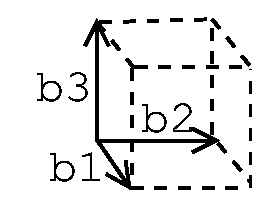
\includegraphics{lattice-vectors.eps}
\caption{Lattice vectors (\matvec{b_1},\matvec{b_2},\matvec{b_3}) that
define the unit cell in a periodic solid.}
\label{lattice-vectors}
\end{center}
\end{figure}

\section{Energy Bands}
We know from our earlier studies that when we use quantum mechanics to
atoms or molecules we obtain a discrete set of states. Solids contain
on the order of $10^{23}$ atoms, and consequently these discrete
states are blurred into \emph{bands}.

\begin{figure}
\begin{center}
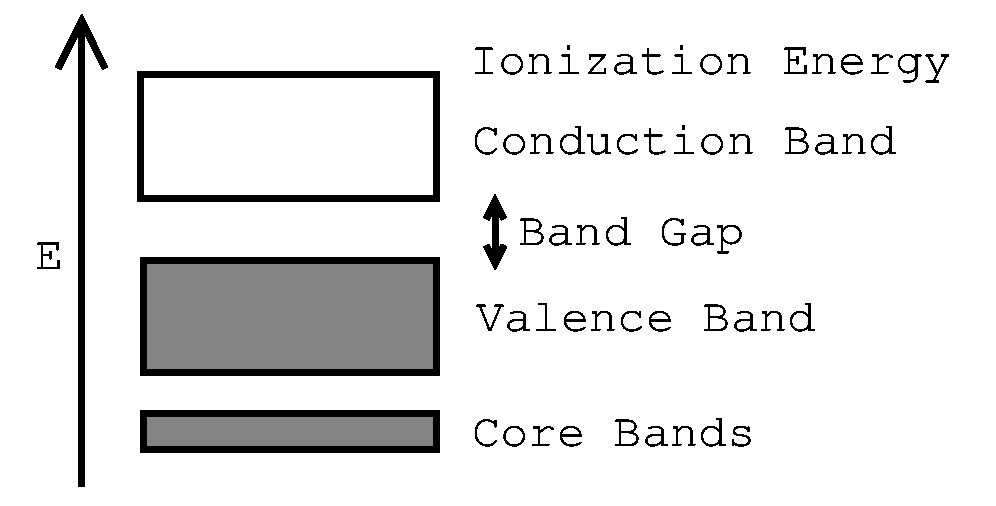
\includegraphics[scale=0.5]{E_Bands.eps}
\caption{Schematic drawing of energy bands in an insulator.}
\label{e-bands-fig}
\end{center}
\end{figure}

Figure \ref{e-bands-fig} shows a schematic drawing of energy bands in
an insulating solid. The gray shading of the core and valence bands
indicates that these bands are occupied, and the lack of shading of the
conduction band indicates that this band is empty. There is a finite
energy gap between the highest occupied electron energy (known as the
\emph{valence band maximum} in solids) and the lowest unoccupied
electron energy (known as the \emph{conduction band minimum}). Since
the valence band is fully occupied, there are no easily accessible
states for an electron in the valence band, which means that to move
around the crystal, the electron needs to be excited into the
conduction band to move around, which requires a finite amount of
energy. This energy requirement is why insulators do not conduct
electricity; given energy they can conduct, which is why insulators
are also known as \emph{semiconductors}. Table \ref{band-gaps-table}
presents the band gaps of well-known semiconductors.

\begin{table}
\begin{center}
\caption{Band gaps of well-known semiconductors.}
\label{band-gaps-table}
\begin{tabular}{ll}\\ \hline\hline
Semiconductor & Band Gap (eV) \\ \hline
C (diamond) & 5.4 \\
Si & 1.17 \\
Ge & 0.74 \\
SiC & 2.8 \\
GaN & 3.5 \\
GaP & 2.32 \\
GaAs & 1.52 \\
InP & 1.42 \\
InAs & 0.43 \\
\hline\hline
\end{tabular}
\end{center}
\end{table}

\begin{figure}
\begin{center}
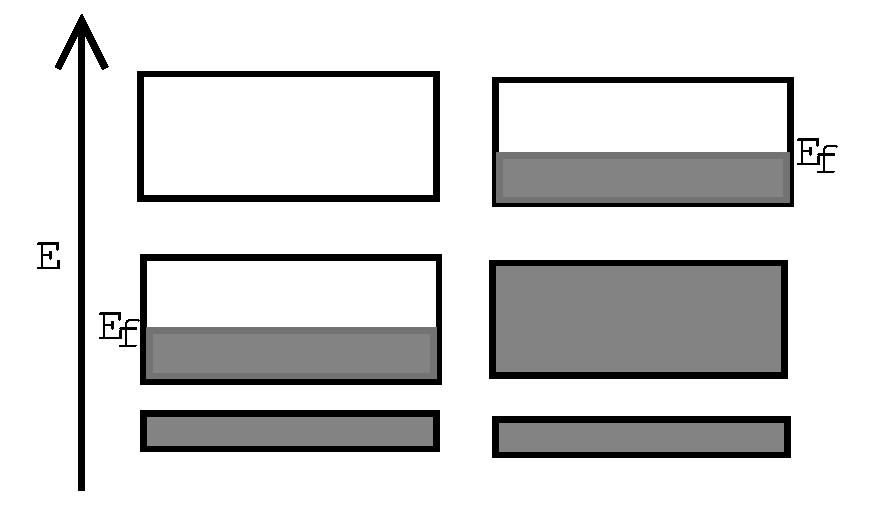
\includegraphics[scale=0.5]{E_Bands_Metal.eps}
\caption{Schematic drawing of different fillings of the energy bands
in a metal.} 
\label{e-bands-metal-fig}
\end{center}
\end{figure}

Figure \ref{e-bands-metal-fig} shows analogous filling of the energy
bands for a metallic solid. In a metal the highest occupied band is
only partially filled, and there are accessible states for electrons
in the valence band. The fact that metals do not have a band gap like
semiconductors do is why metals can conduct electrons: no additional
energy is required to move an electron to an adjacent state. The
\emph{Fermi level} or \emph{Fermi energy} $E_f$ is the energy of the
highest occupied electron, and is labeled in each figure.

The next section will begin to explore the reasons why states in solid
localize into bands.

\begin{figure}
\begin{center}
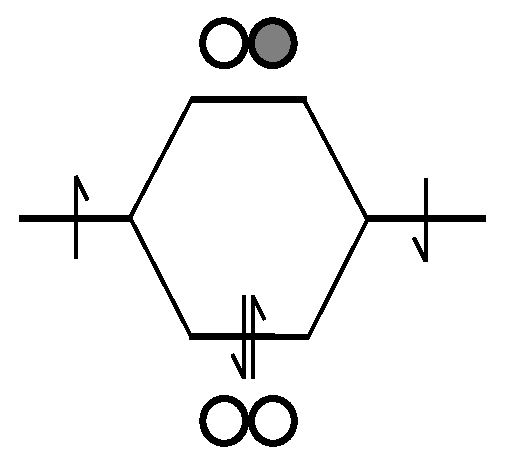
\includegraphics[scale=0.6]{h2-bonding.eps}
\caption{The bonding of two H $1s$ orbitals to make bonding $\sigma_g$
and antibonding $\sigma_u$ orbitals.}
\label{h2-bonding}
\end{center}
\end{figure}

\section{One-Dimensional Periodic Arrays of Atoms}
We already know that the lowest energy state of a hydrogen atom is a
$1s$ orbital. When we bond two hydrogen atoms together we form a
bonding $\sigma_g$ state and an antibonding $\sigma_u$ state; the two
electrons from the H atoms will doubly occupy the $\sigma_g$ state. 
Figure \ref{h2-bonding} shows this interaction.

\begin{figure}
\begin{center}
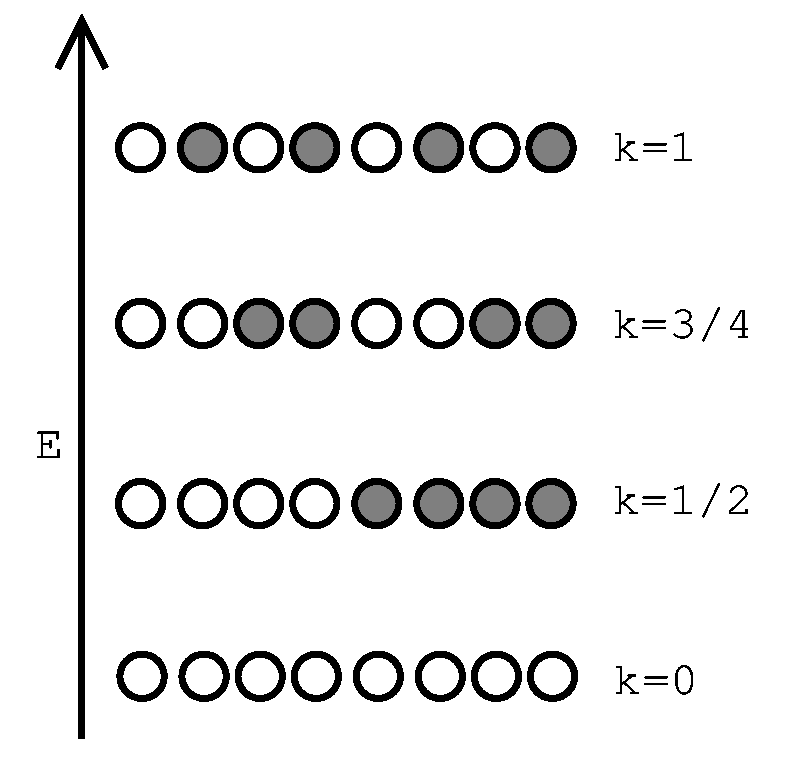
\includegraphics[scale=0.5]{1d-chains.eps}
\caption{Different states that 8 H atoms can have in a one-dimensional
chain, indexed by the $k$-number.}
\label{1d-chains}
\end{center}
\end{figure}

What happens when we take chains of hydrogen atoms? We can think of a
single hydrogen atom as our unit cell that will be translated in one
dimension. Figure \ref{1d-chains} shows different states that eight H
atoms can have. We may approximate the wave function of this system by
\begin{equation}
 \phi(x+X) = \phi_{1s}(x)\cos\left(\frac{2\pi}{a}kx\right).
\label{h-bloch}
\end{equation}
Here $\phi_{1s}$ is the $1s$ wave function for an isolated H atom. $a$
is the lattice spacing between the unit cell images. The
lowercase coordinate $x$ refers to the coordinate within a unit cell,
and the uppercase coordinate $X$ refers to the coordinates between
unit cells. The $k$-number is a measure of how much the phase changes
from one unit cell to the next: when $k=0$ the unit cells are always
replicated with the same sign and when $k=1$ the unit cells alternate
signs. 

\begin{figure}
\begin{center}
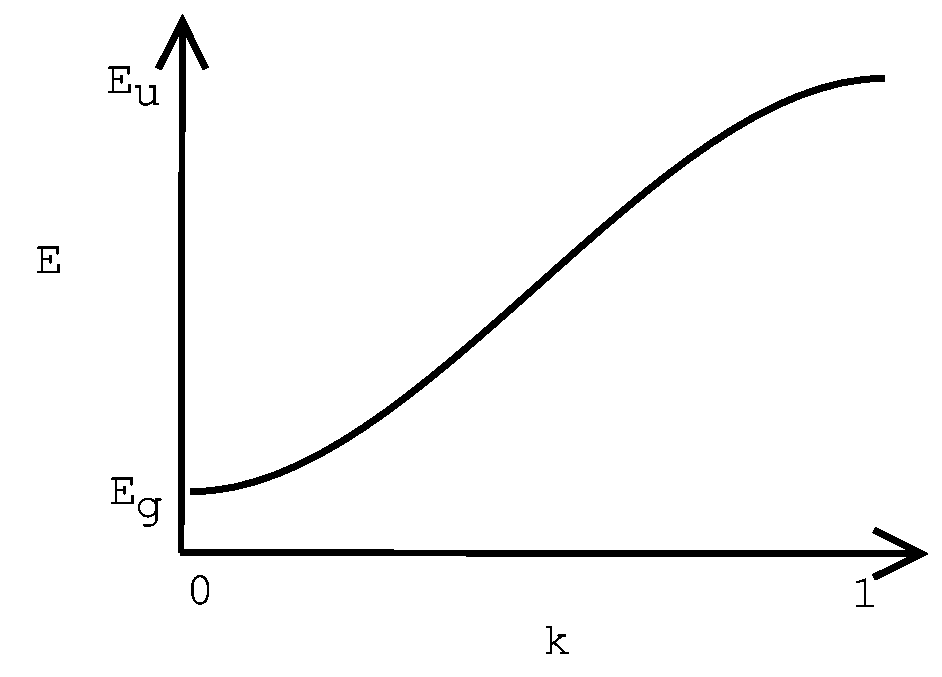
\includegraphics[scale=0.5]{1d-EvsK}
\caption{The variation of the energy with the $k$-number for a simple
one-dimensional chain of H atoms.}
\label{1d-EvsK}
\end{center}
\end{figure}

What is remarkable about the $k$-number is that we can boil bonding
configurations, antibonding configurations, and everything in between,
down to a single parameter. We will find it useful to consider the
energy as a function of the $k$-number, as shown in Figure
\ref{1d-EvsK}, which shows how the single energy band varies from the
bonding to the antibonding limit with the variable $k$. 

Since we have one H atom in each unit cell, we only have one electron
in the band, which means that the band will be half-filled: the
$k$-states from 0--1/2 will be occupied, and the $k$-states from
1/2--1 will be unoccupied. Since there is no gap between occupied and
the unoccupied regions, we would predict that this is a metallic
system.

\begin{figure}
\begin{center}
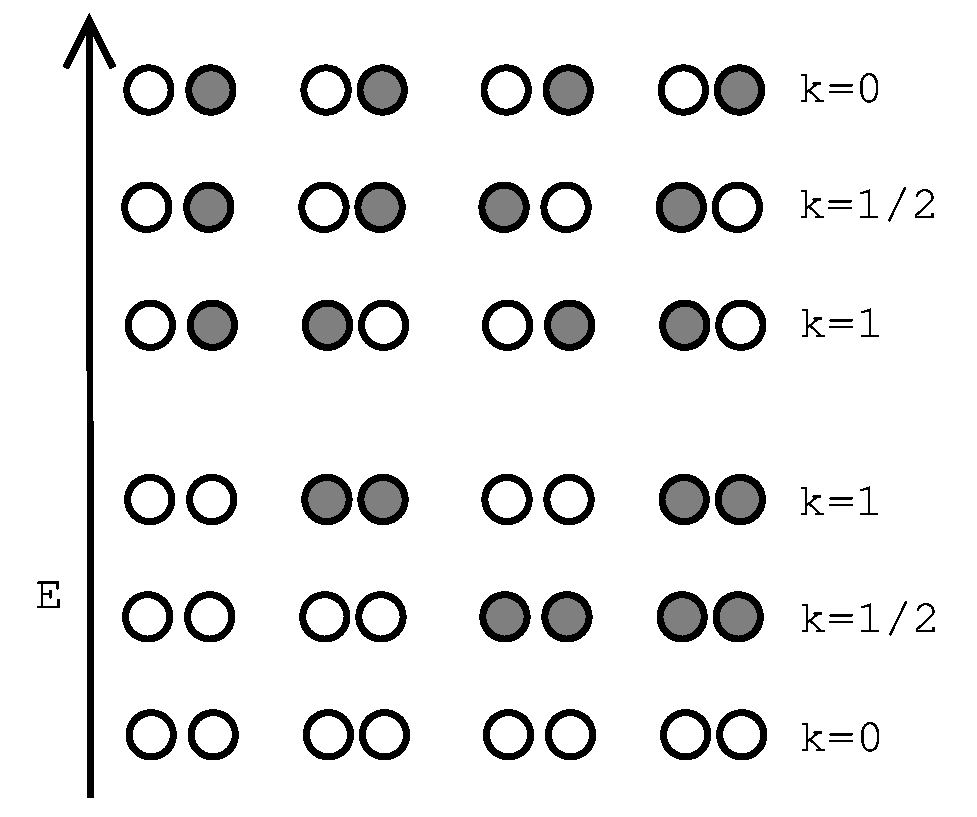
\includegraphics[scale=0.5]{1d-h2-states.eps}
\caption{States of the doubled unit cell with a \chem{H_2} molecule in
each unit cell.}
\label{1d-h2-states}
\end{center}
\end{figure}

\begin{figure}
\begin{center}
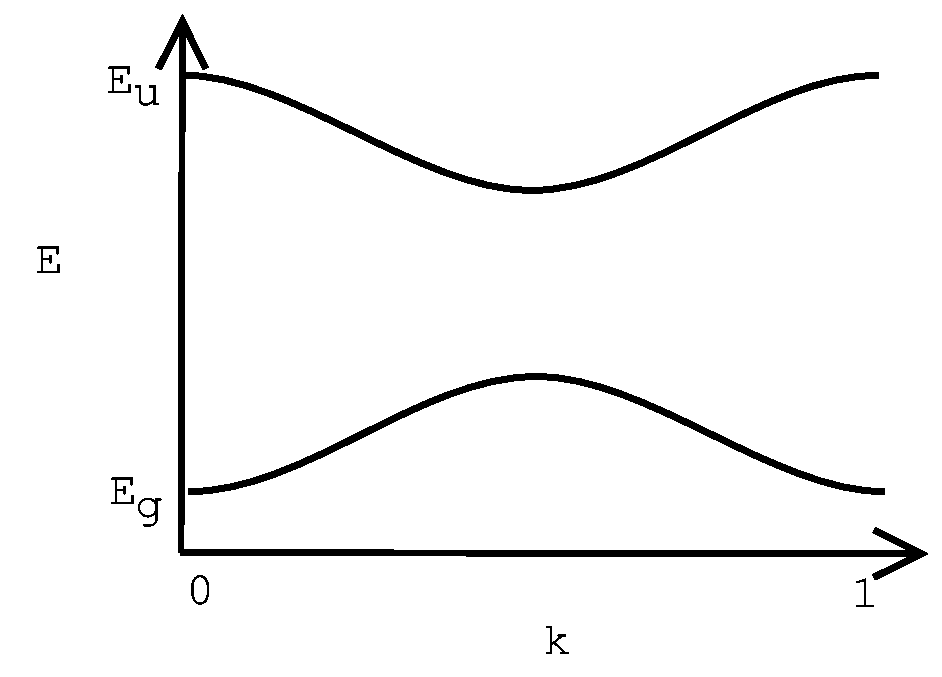
\includegraphics[scale=0.5]{1d-h2-bands.eps}
\caption{Band structure of the doubled unit cell with a \chem{H_2}
molecule in each unit cell.}
\label{1d-h2-bands}
\end{center}
\end{figure}

How do we make insulating systems? We can look again at our poly-H
example, but this time we will \emph{double} the unit cell and put a
bonded \chem{H_2} in each cell. The wave function for the valence band
is
\begin{equation}
 \phi_v(x+X) = \sigma_g(x)\cos\left(\frac{2\pi}{a}kx\right),
\label{h2g-bloch}
\end{equation}
and the wave function for the conduction band is
\begin{equation}
 \phi_c(x+X) = \sigma_u(x)\cos\left(\frac{2\pi}{a}kx\right).
\label{h2u-bloch}
\end{equation}
The variation of these states is
shown in Figure \ref{1d-h2-states} and the energy of the resulting
bands is shown in Figure \ref{1d-h2-bands}. Since we now have two
electrons in each unit cell, we can doubly occupy the lower band, and
keep the upper band unoccupied. This configuration leads to an
insulating system, since there is a finite band gap between the
occupied valence band and the unoccupied conduction band.

In the beginning of the chapter when we were describing how single
orbital states were broadened into energy bands we talked about them
being \emph{smeared out}. This simple example shows us that the
process is really much more precise. We can combine the unit cells
with  different translational symmetries, and these different
symmetries have different energies. The $k$-number is a useful way to
index the translational symmetries.

\begin{figure}
\begin{center}
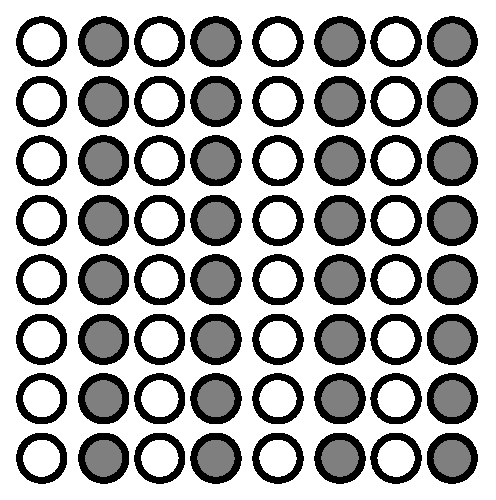
\includegraphics[scale=0.5]{2d-states.eps}
\caption{A two dimensional plane of H atoms with a $k$-state (1,0).}
\label{2d-states}
\end{center}
\end{figure}

The concept of $k$ states is also useful when we have systems that are
periodic in more than one dimension. Figure \ref{2d-states} shows a
two dimensional plane of H atoms, with a $k$-state of (1,0). When we
have a three-dimensional system we specify $(k_x, k_y, k_z)$
states. The next section expands on this idea more.

\section{Reciprocal Space and Brillouin Zones}
The previous system shows that looking at the behavior of the orbital
versus the $k$-vector can give us information about how the entire
energy band works. We can think of the $k$-space $(k_x,k_y,k_z)$
spanned by all possible $k$-vectors as the Fourier transform of the
real $(x,y,z)$ space. This space is known as \emph{reciprocal space}.

The reciprocal space \matvec{d} satisfies
\begin{equation}
 \matvec{b}\cdot\matvec{d}=2\pi.
\end{equation}
These vectors are given by
\begin{equation}
 \matvec{d_j} = \pm2\pi\frac{\matvec{b_k}\times\matvec{b_l}}
                {\matvec{b_1}\cdot(\matvec{b_2}\times\matvec{b_3})}
\end{equation}
where the $+$ sign goes with even permutations of $jkl$, and the $-$
sign goes with odd permutations.

The (first) \emph{Brillouin zone} is the reciprocal space
transform of the unit cell. Just as we will have to integrate over all
points in the unit cell to perform a real space integration, we will
have to integrate over all points in the Brillouin zone to perform a
reciprocal space integration. By understanding the behavior of the
energy bands across the Brillouin zone we may understand all of the
electronic properties of the crystal.

In Figures \ref{1d-EvsK} and \ref{1d-h2-bands} we looked at how the
energy varied with the $k$-state across a band. Unfortunately, for
periodicities higher than 1, we can't put together a simple plot like
this. What we typically do is define \emph{special points} in the
Brillouin zone:
\begin{description} 
\item[$\Gamma$] is defined as (0,0,0); 
\item[X] is defined as (1,0,0); 
\item[K] is defined as (3/4,3/4,0);
\item[W] is defined as (1,1/2,0);
\item[L] is defined as (1/2,1/2,1/2).
\end{description}
We can then describe the variation of the electronic structure of the
entire Brillouin zone by sampling $k$-points that connect these
special points. That is, by sampling the band
structure from $\Gamma$ to $X$ to $W$ to $L$ back to $\Gamma$ to $K$
we can understand the behavior of bands over the entire Brillouin
zone. Figure \ref{si-band} shows such a band structure.

\section{Bloch's Theorem}
The one-dimensional equations \ref{h-bloch}--\ref{h2u-bloch} for the
periodic wave function may be generalized to higher dimensions.
Bloch worked out the solution for the Schrodinger equation in periodic
systems. Bloch proved that solutions of the periodic potential
have the form
\begin{equation}
 \psi(\matvec{k},\matvec{r}) = \mu(\matvec{k},\matvec{r})
    \exp\left(i\frac{2\pi}{a}\matvec{k}\cdot\matvec{r}\right).
\end{equation}
Here the \emph{modulating function} $\mu(\matvec{k},\matvec{r})$ is
the part of the wave function that is the same in every unit cell. The
\emph{phase function} $\exp(i\matvec{k}\cdot\matvec{r})$ multiplies the
modulating function by a wave that has the periodicity of the
crystal. In our simple one-dimensional examples we used a cosine
function, but for mathematical simplicity for real systems we use the
\emph{plane waves} shown here.

\section{Tight Binding Calculations}
\begin{figure}
\begin{center}
\includegraphics[scale=0.5,angle=270]{si_band.eps}
\caption{Band structure of cubic Si using Harrison's tight binding
technique.}
\label{si-band}
\end{center}
\end{figure}

To show an example of how kpoints affect the Hamiltonian in a periodic
calculation, we now discuss a very simple example of such a
calculation. 
Chadi and Cohen \cite{Chadi75} and Harrison \cite{Harrison80} define a
very useful semiempirical technique for doing band calculations on
diamond-like structures such as Si or GaAs. The model Hamiltonian is
defined as:
\begin{equation}
\matvec{H}(\matvec{k})=\left(
\begin{array}{cccccccc}
E_s^c & E_{ss}g_0 & 0 & 0 & 0 & E_{sp}g_1 & E_{sp}g_2 & E_{sp}g_3 \\
E_{ss}g_0 & E_s^a & -E_{sp}g_1^* & -E_{sp}g_2^* & -E_{sp}g_3^* &
  0 & 0 & 0\\
0 & -E_{sp}g_1 & E_p^c & 0 & 0 & E_{xx}g_0 &E_{xy}g_3 &E_{xy}g_2 \\
0 & -E_{sp}g_2 & 0 & E_p^c & 0 & E_{xy}g_3 &E_{xx}g_0 &E_{xy}g_1 \\
0 & -E_{sp}g_3 & 0 & 0 & E_p^c & E_{xy}g_2 &E_{xy}g_1 &E_{xx}g_0 \\
-E_{sp}g_1^* & 0 & E_{xx}g_0^* & E_{xy}g_3^* &E_{xy}g_2^*&
   E_p^a & 0 & 0 \\
-E_{sp}g_2^* & 0 & E_{xy}g_3^* & E_{xx}g_0^* &E_{xy}g_2^*&
   0 & E_p^a & 0 \\
-E_{sp}g_3^* & 0 & E_{xy}g_2^* & E_{xy}g_1^* &E_{xx}g_0^*&
   0 & 0 &E_p^a 
\end{array}
\right)
\label{harrison-ham}
\end{equation}
With the Hamiltonian in this form, one must solve
\begin{equation}
\matvec{H}(\matvec{k})\matvec{c}(\matvec{k}) 
  = E(\matvec{k})\matvec{c}(\matvec{k})
\end{equation}
where the values of \matvec{k} extend over the whole Brillouin zone.
The terms $E_s^c$, $E_{ss}$, $E_{xx}$, $E_{xy}$ are parameters
fit for each different material. The superscript $c$ refers to the
\emph{cation}, that is, the column 3 element in a 3,5 semiconductor,
or the column 2 element in a 2,6 semiconductor; the superscript $a$
refers to the \emph{anion}, the other species in each of these. Of
course, for a pure semiconductor like Si, Si is both the cation and
the anion.

The phase factors $g_0$, $g_1$, $g_2$, $g_3$ determine how the
Hamiltonian changes across the Brillouin zone. These are given by 
\begin{equation}
 g_0(\matvec{k}) = \exp(i\matvec{k}\cdot\matvec{d_1})
    + \exp(i\matvec{k}\cdot\matvec{d_2})
    + \exp(i\matvec{k}\cdot\matvec{d_3})
    + \exp(i\matvec{k}\cdot\matvec{d_4})
\end{equation}
\begin{equation}
 g_1(\matvec{k}) = \exp(i\matvec{k}\cdot\matvec{d_1})
    + \exp(i\matvec{k}\cdot\matvec{d_2})
    - \exp(i\matvec{k}\cdot\matvec{d_3})
    - \exp(i\matvec{k}\cdot\matvec{d_4})
\end{equation}
\begin{equation}
 g_2(\matvec{k}) = \exp(i\matvec{k}\cdot\matvec{d_1})
    - \exp(i\matvec{k}\cdot\matvec{d_2})
    + \exp(i\matvec{k}\cdot\matvec{d_3})
    - \exp(i\matvec{k}\cdot\matvec{d_4})
\end{equation}
\begin{equation}
 g_3(\matvec{k}) = \exp(i\matvec{k}\cdot\matvec{d_1})
    - \exp(i\matvec{k}\cdot\matvec{d_2})
    - \exp(i\matvec{k}\cdot\matvec{d_3})
    + \exp(i\matvec{k}\cdot\matvec{d_4})
\end{equation}
where the lattice vectors for a diamond structure are given by
\begin{equation}
 \matvec{d_1} = (1,1,1)a/4
\end{equation}
\begin{equation}
 \matvec{d_2} = (1,\bar{1},\bar{1})a/4
\end{equation}
\begin{equation}
 \matvec{d_3} = (\bar{1},1,\bar{1})a/4
\end{equation}
\begin{equation}
 \matvec{d_4} = (\bar{1},\bar{1},1)a/4
\end{equation}
and $a$ is the lattice constant.

A sample band structure for Si is shown in Figure \ref{si-band}. In a
tight binding calculation of this type, one performs the following
steps.
\begin{enumerate}
 \item Form the constants $E_s^c$, $E_{ss}$, $E_{xx}$, $E_{xy}$ based 
	on the cation and anion specified in the problem.
 \item For each \emph{kpoint} \matvec{k_i} in the Brillouin zone:
 \begin{enumerate}
   \item Form the Hamiltonian $H(\matvec{k_i})$ from equation
	\ref{harrison-ham}.
   \item Diagonalize the $H(\matvec{k_i})$ and save the energies
	$\{E(\matvec{k_i})\}$.
 \end{enumerate}
 \item Form the band structure by connecting the adjacent points of 
	$\{E(\matvec{k_i})\}$ for all kpoints in the Brillouin zone.
\end{enumerate}

Simple programs to compute tight-binding band structures using this
method are available at 
\href{http://wag.caltech.edu/home/rpm/project/tight-binding}
     {http://wag.caltech.edu/home/rpm/project/tight-binding}.

%\section{Augmented Plane Wave Calculations}

\section{Plane Wave DFT Calculations}
The majority of electronic structure calculations that employ periodic
boundary conditions use density functional theory calculations with
plane waves and pseudopotentials. Several features make plane waves
desirable. Plane waves are already periodic functions, and so they are
a natural choice for use as basis functions on systems that are also
periodic. Furthermore, computing the one- and two-electron integrals
is much easier using plane waves, where most of the integrals are
zero, than any other type of basis function. 

However, several aspects of plane waves make them problematic. The
first is that many more plane wave basis functions are required to
describe an atom than would be required using, for example, Gaussian
basis functions. One can perform a good calculation on water using a
6-31G** basis set with only 25 basis functions. The same level of
accuracy using plane waves requires well over 1000 plane wave
functions. Although, as we already noted, Hamiltonian matrix elements
are much easier to compute using plane waves than using Gaussians, one
still must determine the eigenfunctions of the Hamiltonian, a process
which is time consuming for matrices of this size.

The second problem with plane waves is their inability to describe
local phenomena. Fourier expansions of smooth, delocalized functions
require far fewer plane waves than sharp, localized functions. To keep
the basis set size from getting enormous, plane waves higher than a
certain angular momentum are typically excluded from the basis
set. One of the effects of this exclusion is that plane waves cannot
describe core electrons. Typically this is not a terrible problem,
because \emph{pseudopotentials} (also known as \emph{effective core
potentials}) are typically used to remove the core electrons so that
the plane waves need only describe the valence electrons. However,
this often requires using core potentials for atoms like carbon that
are not always well described with these functions. Nonetheless, in
general the replacement of core electrons with pseudopotentials is an
accurate and a straightforward process. 

However, the inability of plane waves to describe localized phenomena
is potentially a difficulty when describing chemical processes that
might themselves be localized. The bonding of an adatom to a metal
surface will typically be highly localized, and it is not always
practical to add enough basis functions to properly describe
it. Similarly, when PBC code is used to describe finite systems (the
\emph{supercell} method, where the molecule is put in a large enough
unit cell to keep it from seeing its periodic neighbors), rarely are
enough functions used to describe the molecule adequately.

For most solid systems, however, plane waves do an adequate job of
describing the electronic structure.
The next section describes attempts to use localized Gaussian functions in
calculations using periodic boundary conditions to circumvent the
problems plane waves have.

\section{Gaussian Basis Set DFT Calculations}
Techniques using Gaussian basis sets in density functional theory
calculations on systems with periodic boundary conditions are
currently under development. These calculations work by using a
combination of spherically symmetric \emph{reference atoms} to
describe the electron density around each atom. The reference atoms
are defined by specifying a linear combination of Gaussian basis
functions, and must be accurate enough that whatever is omitted is a
slowly varying function. This remainder density may then be described
using a very sparse set of plane wave functions. The SeqQuest program
developed at Sandia National Laboratories with help from the Caltech
Materials and Process Simulation Center uses this approach.

%\section{Example: Diamond and Graphite}

\section{Suggestions for Further Reading}
Kittel's \emph{Introduction to Solid State Physics} \cite{Kittel53}
presents a complete introduction to the field of solid state
physics. Harrison's \emph{Electronic Structure and the Properties of
Solids} \cite{Harrison80} gives a good overview of tight binding
calculations for solids. The classic paper on this method is Slater
and Koster 1954 Physical Review paper \cite{Slater54}. Martin and
Leonard's \emph{Electrons and Crystals} \cite{Martin70} presents a
good general discussion on the electronic properties of solids, but is
regrettably out of print. Thijssen's excellent book
\emph{Computational Physics} \cite{Thijssen99} has a good chapter on
periodic boundary conditions.

\chapter{Parameters for Chemical Kinetics Calculations}

\graphicspath{{./Figures/Kinetics/}}

\section{Introduction to Chemical Kinetics} 
Chemical kinetics calculations are a very useful way to take quantum
chemical results and compare the predictions to experimental
results. With kinetics software one can predict the evolution of large
mixtures of reactants over time, can model combustion and detonation
processes, and can predict equilibrium mixtures. 

In kinetics we're interested in how fast chemical reactions run. Given
a reaction, for example,
\begin{equation}
 \chem{Br} + \chem{H_2} \rightleftharpoons \chem{HBr} + \chem{H},
\end{equation}
how fast are the products (\chem{HBr}) produced? Using simple
kinetics, we can write the rate of product production as a function of
a \emph{rate constant} times the concentrations of the reactants:
\begin{equation}
 \frac{\partial [\chem{HBr}]}{\partial t} =
  k[\chem{Br}][\chem{H_2}].
\end{equation}
For simple reactions like this it is easy to work out the kinetic
equations, and even to integrate them given different starting
conditions. However, reaction networks become complex very
rapidly. The combustion of hydrogen and oxygen to produce water
\begin{equation}
 \chem{H_2} + \chem{O_2} \rightleftharpoons \chem{H_2O}
\end{equation}
has 10 elementary reactions in it. People who model hydrocarbon
combustion routinely deal with reaction networks that have thousands
of reactions. As reaction networks become more complex, we need to use
computer programs to integrate all of the variables
simultaneously. The first part of this chapter discusses the software
used in these simulations and what types of parameters it
requires. The second part of this chapter then examines how quantum
chemistry calculations may be used to determine these parameters.

\section{The Chemkin program and associated parameter files} 
The most commonly used chemical kinetics program is the Chemkin
package, originally developed by Sandia National Laboratories
\cite{chemkin2}, and currently marketed by Reaction Design. Two free
alternatives to the Chemkin package are Cantera \cite{Goodwin02} and
Fuego \cite{Aivazis02}, both being developed at Caltech. Of these
efforts, Cantera is the most mature, and information on the status of
the program may be found at the Cantera web site
\href{http://www.cantera.org}{http://www.cantera.org}.

Given a collection of species \chem{X_1}, \chem{X_2}, \dots, at
concentrations [\chem{X_1}], [\chem{X_2}], \dots and a given
temperature $T$ and pressure $P$, Chemkin determines the rate of
change of these variables $\frac{\partial[\chem{X_i}]}{\partial t}$,
$\frac{\partial T}{\partial t}$, $\frac{\partial P}{\partial
t}$. Although this may seem very straightforward, it enables one to
take a set of initial conditions, and, for example, simulate the
detonation of explosive materials over time, as shown in Figure
\ref{hmx-species}.

\begin{figure}
\begin{center}
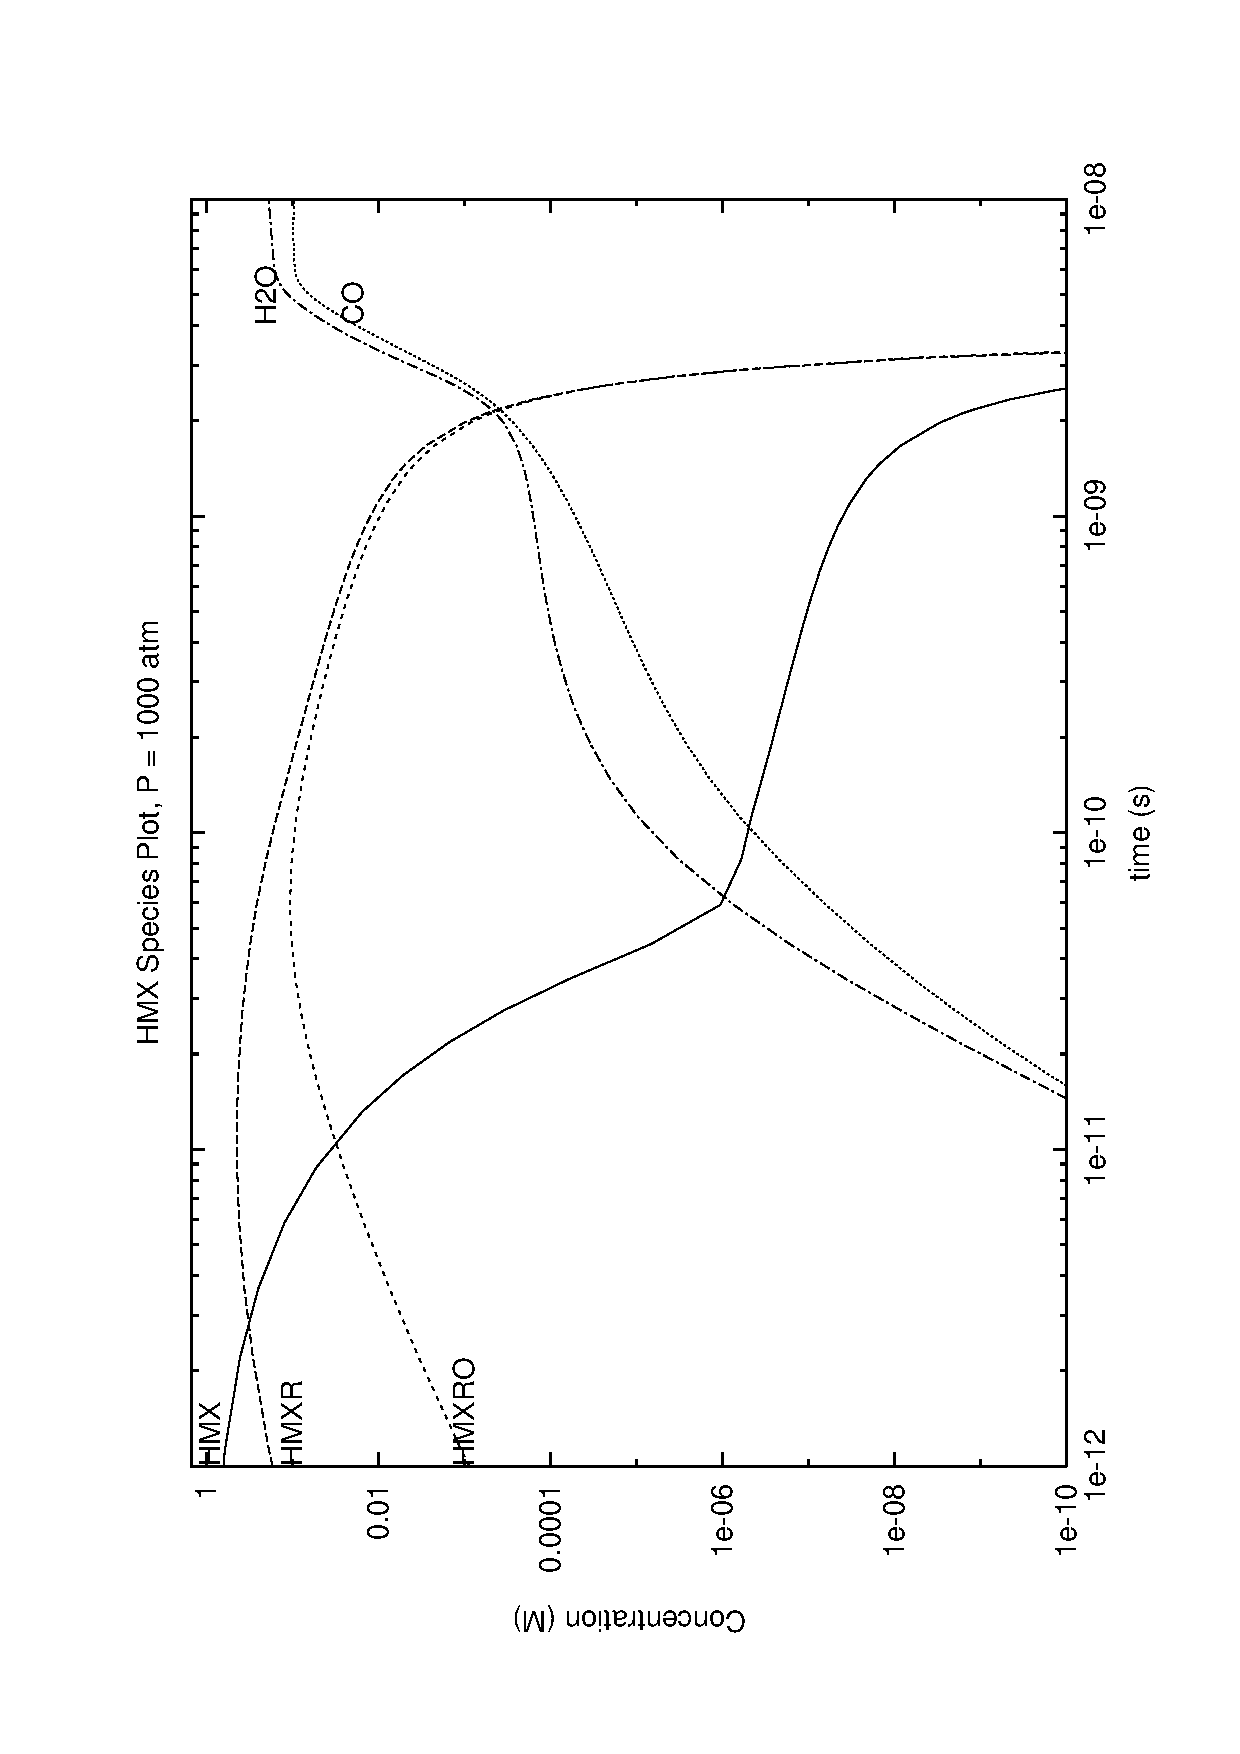
\includegraphics[angle=270,scale=0.5]{hmx-species}
\end{center}
\caption{Detonation of the explosive material HMX over time, computed
using a Chemkin constant volume calculation at P=1000 atm and T=1500
K. The material detonates at $\approx 2\times 10^{-9}$ sec. The
mechanism used to study this process contains over 90 species and 450
reactions, and thus requires a computer program to simulate.}
\label{hmx-species}
\end{figure}

A Chemkin mechanism file has four sections: (i) an elements section
that lists the relevant elements in the reaction; (ii) a species
section that lists all of the species; (iii) a thermochemistry section
that contains composition and thermochemical information for each of
the species; and (iv) a reactions section that describes kinetic
parameters for each reaction.

An example of a species entry for the thermochemistry section is
\begin{verbatim}
C2H2              121386C   2H   2      G  0300   5000  1000  
 0.04436E+02 0.05376E-01-0.01912E-04 0.03286E-08-0.02156E-12
 0.02566E+06-0.02800E+02 0.02013E+02 0.01519E+00-0.01616E-03
 0.09078E-07-0.01912E-10 0.02612E+06 0.08805E+02               
\end{verbatim}
This record is for acetylene, \chem{C_2H_2}. The first record is the
name of the species, and the second record (121386) is an (arbitrary)
identifying number, generally the date on which the data was
generated. The next four records (\verb:C   2H   2:) indicate that
there are 2 carbon and 2 hydrogen atoms in this species. The next
record (\verb:G:) indicates that the species is gaseous, and the next
three records say that the thermochemical data is fit from 300--5000
K, and that the turnover point from the low-temperature to the
high-temperature regime is 1000 K.

The next 14 records are parameters for the \emph{NASA thermochemical
polynomial fit} to the thermochemical data, given by
\begin{eqnarray}
C_p/R &=& a_1 + a_2T + a_3T^2 + a_4T^3 + a_5T^4\\
H/RT &=& a_1 + a_2T/2 + a_3T^2/3 + a_4T^3/4 + a_5T^4/5 + a_6/T\\
S/R &=& a_1\ln T + a_2T + a_3T^2/2 + a_4T^3/3 + a_5T^4/4 + a_7
\end{eqnarray}
The first 7 records contain $a_1$--$a_7$ for the high temperature
range, and the next 7 records contain $a_1$--$a_7$ for the low
temperature range.  To determine parameters for these polynomials, the
techniques of Chapter \ref{chap-thermochem} are used to compute the
heat capacity $C_p$, the enthalpy $H$, and the entropy $S$ over a wide
range of temperatures. These data are then fit using a standard set of
programs to the NASA thermochemical form. Figure \ref{hmx-therm} shows
representative data for the energetic material HMX and the NASA fit to
these data.

\begin{figure}
\begin{center}
\includegraphics[scale=0.5,angle=270]{hmx.eps}
\end{center}
\caption{HMX molecule thermodynamic data for $C_p$ and $S$ from DFT
calculation (points) and fit to NASA polynomial (lines), in cal/mol K.}
\label{hmx-therm}
\end{figure}

\begin{table}
\caption{Examples of reaction parameters in a Chemkin mechanism.}
\label{chemkin-reaction}
\begin{center}
\begin{tabular}{llll}\hline\hline
Reaction & A & $\beta$ & $E_a$ \\ \hline
$\chem{O}+\chem{H_2}\rightleftharpoons \chem{H}+\chem{OH}$       
 & 5.000E+04 &  2.670 &  6290.00\\
$\chem{O}+\chem{HO_2}\rightleftharpoons \chem{OH}+\chem{O_2}$     
 & 2.000E+13 &   .000 &      .00\\ 
$\chem{O}+\chem{H_2O_2}\rightleftharpoons \chem{OH}+\chem{HO2}$   
 & 9.630E+06 &  2.000 &  4000.00\\
\hline\hline
\end{tabular}
\end{center}
\end{table}


Table \ref{chemkin-reaction} shows typical reactions from the
reactions section of the Chemkin file. The basic information contains
the species in the reaction, and $A$, $\beta$, and $E_a$ parameters
for the \emph{modified Arrhenius equation}
\begin{equation}
 k=AT^\beta\exp\{-E_a/k_bT\}
\end{equation}
where $A$ is the \emph{pre-exponential factor}, $T$ is the temperature
of the reaction, $\beta$ is the temperature exponent, $E_a$ is the
\emph{activation energy}, and $k_b$ is Boltzmann's constant.

In many dissociation or recombination reactions a \emph{third body} is
required to carry off excess kinetic energy. In Chemkin reactions
these processes are normally written as
\begin{equation}
 \chem{H} + \chem{O_2} + \chem{M} \rightleftharpoons \chem{HO_2} + \chem{M}
\end{equation}
where the species \chem{M} represents a generic third body species. It
is often the case that some species act more efficiently than others
as a third body, and then the \emph{third body efficiency} is
specified as, for example,
\begin{verbatim}
 H2/ 2.40/ H2O/15.40/ CH4/ 2.00/
\end{verbatim}

Another type of specification commonly made in Chemkin mechanism files
is the \emph{pressure-dependent fall-off reaction}
parameters. Consider the recombination reaction of two methyl
radicals. In the high-pressure regime, the appropriate reaction is
$\chem{CH_3}+\chem{CH_3}\rightleftharpoons\chem{C_2H_6}$. In the
low-pressure regime, the appropriate reaction is 
$\chem{CH_3}+\chem{CH_3}+\chem{M}\rightleftharpoons\chem{C_2H_6}+M$.
The regime between these two limits is known as the fall-off regime.
Chemkin keywords \verb:LOW: and \verb:TROE: specify parameters for
different types of treatments of these regimes.

%Constant Volume calculations

%Sensitivity analysis

\section{Conventional Transition State Theory}
We now want to understand how to use the quantum chemistry techniques
we have developed in this course to compute parameters to be used in
chemical kinetics calculations.
How can we go from static
properties of the energy at different geometries to obtain intuition
about the reaction dynamics of the system? We will use conventional
transition state theory (CTST). CTST is built upon four major
assumptions
\begin{enumerate}
\item Molecular systems that have surmounted the saddle point in the
direction of products cannot turn back and form reactants again.
\item The energy distribution among the reactants follows the
Maxwell-Boltzmann distribution, and thus the concentration of
activated complexes may be computed from equilibrium theory.
\item The motion along the reaction path is separable from the other
motions of the activated complex.
\item A chemical reaction may be treated classically, with quantum
effects such as tunneling ignored.
\end{enumerate}
There are many different ways to express CTST. The way that we will
find the most convenient is known as the \emph{thermodynamic
formulation}. 
\begin{equation}
 k = \frac{k_BT}{h}\exp\{-\Delta G^\ddag/RT\}
\label{tst}
\end{equation}
Here $k_B$ is the Boltzmann constant ($1.38066\times 10^{-23}
JK^{-1}$), $T$ is the temperature, $h$ is Planck's constant
($6.62618\times 10^{-34} Js$), $R$ is the ideal gas constant ($2 cal
mol^{-1}K^{-1}$), and $\Delta G^\ddag$ is the free energy change
between the ground state and the transition state. The prefactor
$\frac{k_BT}{h}$ has units of $s^{-1}$, and we can think of it as how
rapidly the reactant tries to cross the barrier. The exponential term
$\exp\{-\Delta G^\ddag/RT\}$ is dimensionless, and we can think of it
as how easy it is to get over the barrier. When we multiply the two
terms together we get a good estimate of the ease at which the barrier
may be crossed.


\begin{figure}
\begin{center}
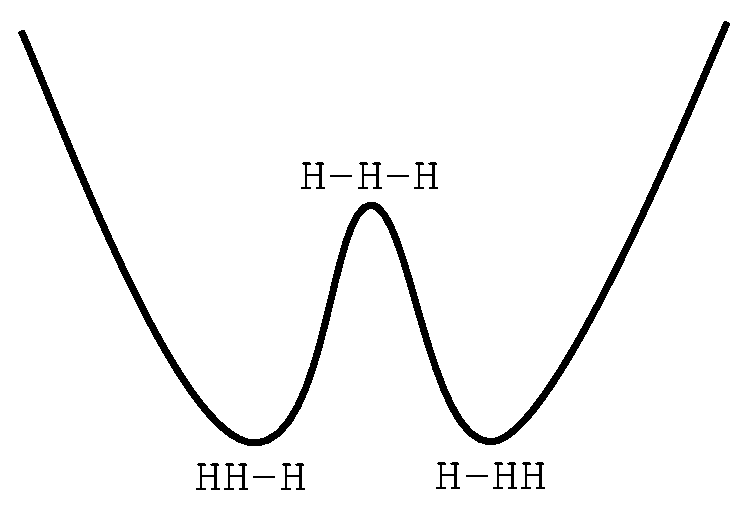
\includegraphics[scale=0.5]{h3-isom.eps}
\end{center}
\caption{Schematic drawing of the \chem{H_2}+\chem{H} atom transfer reaction.}
\label{h3-isom}
\end{figure}

As an example of how CTST may be used, we consider the reaction
$\chem{H_2}+\chem{H}\rightleftharpoons\chem{H}+\chem{H_2}$, shown
schematically in Figure \ref{h3-isom}. We first compute the ground and
transition state geometries and energies. It turns out that there is
an energy difference of 5.99 kcal/mol between the ground and
transition state. We also use the techniques described in section
\ref{chap-thermochem} to approximate the free energy at a variety of
temperatures. Table
\ref{h3-data-table} presents the raw data that we will use for our
plot.

\begin{table}
\caption{Data for computing kinetics parameters for the
\chem{H_2}+\chem{H} reaction.}
\label{h3-data-table}
\begin{center}
\begin{tabular}{ccccccccc}\\ \hline\hline
$T$ & $E^0$ & $G^0$ & $E^\ddag$ & 
 $G^\ddag$ & $\Delta G^\ddag$& $1000/T$ & $k$ & $\ln(k)$ \\ \hline
0      & 0 & 6.74   & 5.99 & 11.86  & 5.12 \\ 
298.15 & 0 & -3.36  & 5.99 &  3.19  & 6.56  & 3.354 &
 $9.69\times 10^7$ & 18.39    \\ 
398.15 & 0 & -8.01  & 5.99 & -0.54  & 7.47  & 2.512 &
 $6.59\times 10^8$ & 20.31    \\ 
498.15 & 0 & -12.96 & 5.99 & -4.50  & 8.47  & 2.007 &
 $2.00\times 10^9$ & 21.42    \\ 
598.15 & 0 & -18.15 & 5.99 & -8.64  & 9.52  & 1.672 &
 $4.15\times 10^9$ & 22.15    \\ 
698.15 & 0 & -23.54 & 5.99 & -12.94 & 10.60 & 1.432 &
 $6.97\times 10^9$ & 22.66    \\ 
\hline\hline
\end{tabular}
\end{center}
\end{table}


Our goal is to fit these data to an \emph{Arrhenius equation}
\begin{equation}
 k = A\exp\{-E_a/RT\}.
\end{equation}
What we are doing here is effectively removing the temperature
dependence of the preexponential factor in the CTST rate expression.
Because chemists have been doing these calculations since long before
there were computers to analyze them they developed a convenient way
to obtain the relevant factors. One makes an \emph{Arrhenius plot}
whereby $\ln(k)$ is plotted as a function of $1000/T$. The
$y$-intercept of the plot gives $\ln{A}$, and the slope of the plot
gives $E_a/1000R$, which means that we can determine $A$ and $E_a$
with only graph paper and a ruler rather than a computer (but as long
as we have one, we may as well use it). Table \ref{h3-data-table} also
has columns that convert the \chem{H_2}+\chem{H} data to the proper
form for plotting, using equation \ref{tst} to estimate the
rate. Figure \ref{h2-h-arrhen} shows the Arrhenius plot of these data,
along with the straight line fit that yields $E_a=4.42 kcal/mol$ and
$A=1.7\times 10^{11}$. 

\begin{figure}
\begin{center}
\includegraphics[scale=0.5,angle=270]{h2-h-arrhen.eps}
\end{center}
\caption{\chem{H_2}+\chem{H} Arrhenius plot, showing the data from
table \ref{h3-data-table} (points) fit to an Arrhenius equation
(line). The data in this plot yields $E_a=4.42$ kcal/mol and
$A=1.7\times 10^{11}$.}
\label{h2-h-arrhen}
\end{figure}

Before we leave this very simple reaction, let us consider a great
simplification of the preexponential factor that is due to (USC
professor) Sidney Benson. For bimolecular reactions, Benson estimated
that the prefactor was given by
\begin{equation}
 A = \frac{k_BT}{h}\exp\{-\Delta S^\ddag/R\}
\end{equation}
where now $\Delta S^\ddag$ is the entropy change between the reactant
state and the transtition state. Using this approximation for the 
\chem{H_2}+\chem{H} reaction just studied yields a preexponential
factor of $A = 2.3\times 10^{11}$, in remarkable agreement with the
more accurate value.

\begin{figure}
\begin{center}
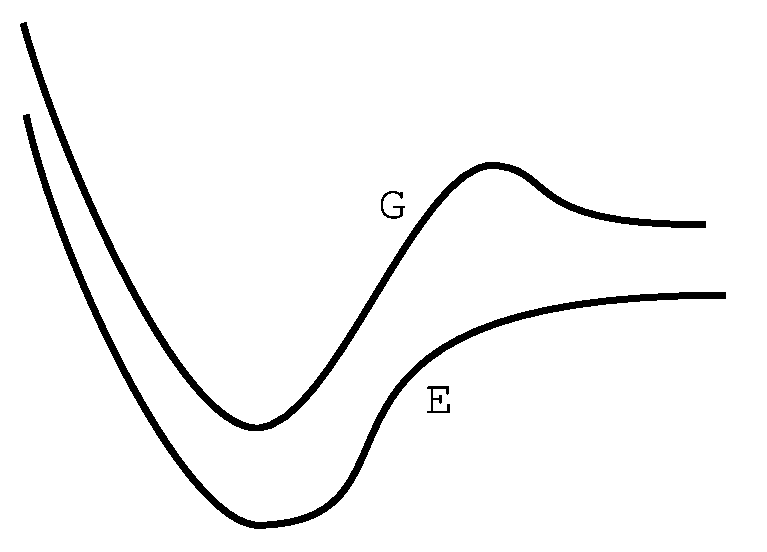
\includegraphics[scale=0.5]{h-recomb.eps}
\end{center}
\caption{The free energy $G$ pathway can have a barrier even for
reactions such as radical recombination where the energy $E$ has no
barrier.}
\label{h-recomb}
\end{figure}

Lorant and Goddard have also shown that we can use transition state
theory techniques to obtain rate constants for barrierless
reactions. Consider the reaction hydrogen atom recombination reaction
$\chem{H} + \chem{H} \rightleftharpoons \chem{H_2}$. The reaction has
no barrier, and traditionally people have assumed that treatment of
this reaction with transition state theory was impossible. Lorant and
Goddard showed that even when the reaction energy had no barrier, it
was still possible to find a barrier along the free energy pathway,
and that the same transition state theory could be used to determine
the rate constants for these reactions. Figure \ref{h-recomb} shows a
(greatly exaggerated) schematic of exactly how this would work. Lorant
and Goddard's technique is a breakthough because it allows rate
constants to be determined for reactions that could only otherwise be
computed using expensive RRKM techniques.

\section{Calculation of Rate Constants for Unimolecular Reactions}
The calculations we discussed in the previous section are
inadequate for describing unimolecular processes. Fortunately, a
number of excellent treatments of unimolecular reactions have been
developed over the years, culminating in RRKM theory, developed by
Rice, Ramsberger, Kassel, and Marcus. A full treatment of RRKM theory
is beyond the scope of the current work, but we will present a brief
overview here.

\begin{figure}
\begin{center}
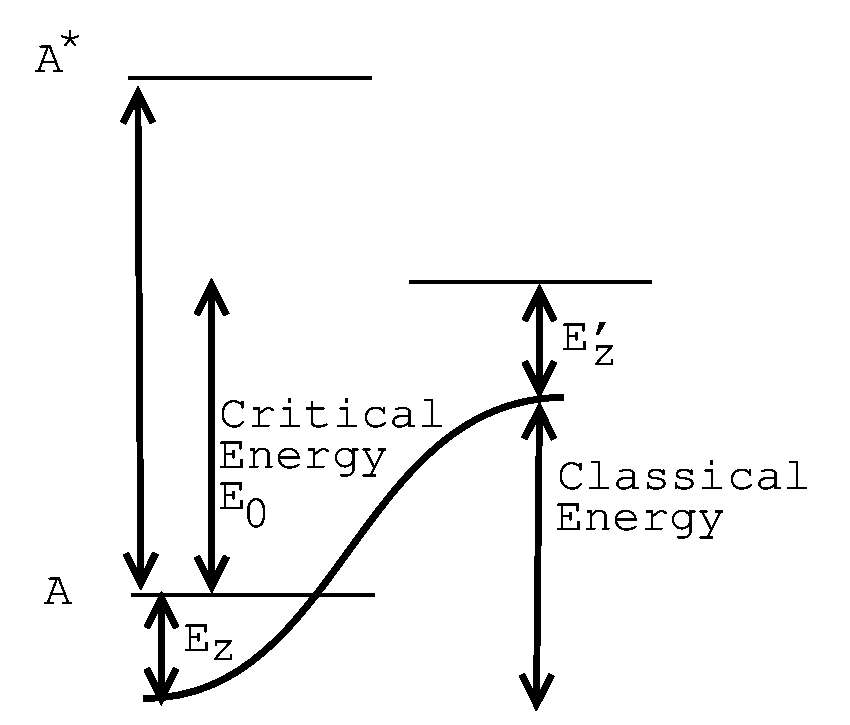
\includegraphics[scale=0.5]{rrkm.eps}
\end{center}
\caption{Energies involved in RRKM calculations. The classical energy
is corrected by the zero-point energies of the ground and transition
states. The molecule \chem{A} is excited to some energized species
\chem{A^*} that has more energy than the critical energy for reaction,
$E_0^*$.}
\label{rrkm}
\end{figure}

RRKM theory assumes that unimolecular reactions proceed according to
\begin{eqnarray}
 \chem{A} + \chem{M} &\stackrel{k_1}{\rightleftharpoons}& 
   \chem{A^*} + \chem{M}\\
 \chem{A^*} &\stackrel{k_2}{\rightarrow}& \chem{B}+\chem{C}
\end{eqnarray}
where the molecule \chem{A} is excited by collision with inert species
\chem{M} to some \emph{energized complex} \chem{A^*} which can then
react to form products \chem{B} and \chem{C}. Figure \ref{rrkm} shows
some the energies that enter into such a process.

By standard steady state theory we could assume
\begin{equation}
 k = \frac{k_2(k_1/k_{-1})}{1+k_2/k_{-1}[M]}.
\end{equation}
In RRKM we recognize that both $k_2$ and $f=k_1/k_{-1}$ are functions
of the energy $E^*$. Thus, in differential form
\begin{equation}
 dk = \frac{k_2(E^*)f(E^*)}{1+k_2(E^*)/k_{-1}[M]}dE^*.
\end{equation}
and in integral form
\begin{equation}
 k = \int_{E_0^*}^{\infty}\frac{k_2(E^*)f(E^*)}{1+k_2(E^*)/k_{-1}[M]}dE^*.
\end{equation}
The distribution function $f(E^*)$ is given by
\begin{equation}
 f(E^*)dE^* = \frac{N(E^*)\exp\{-E^*/kT\}dE^*}
  {\int_0^\infty N(E^*)\exp\{-E^*/kT\}dE^*}
\end{equation}
where $N(E^*)$ is the density of states with energies between $E^*$
and $E^*+dE^*$. The expression for $k_2(E^*)$ is given by
\begin{equation}
 k_2(E^*) = \frac{l^\ddag\sum E_\mathrm{active}^*}{hN(E^*)F_r}
\end{equation}
where $l^\ddag$ is the statistical factor, the ratio of the number of
symmetrically identical products to the number of symettrically
identical reactants, $P(E)$ is the number of rovibrational states of
the activated molecule up to $E$, and $F_r$ is a scaling factor to
account for the fact that the rotations are not the same in the
energized and the activated structures.

The \verb:UNIMOL: program is the most commonly used programs to do
RRKM calculations.


\chapter{Electronic Excited States}

\graphicspath{{./Figures/ExcitedStates/}}

\section{Introduction}
Most of the discussion of quantum chemical calculations thus far has
centered on ground state properties. Quantum chemical techniques can
also be used to compute energies and wave functions for electronically
excited states.

Excited states are most relevant when considering absorption
spectroscopy. Molecules can absorb a photon in the Vis-UV range and
convert to an electronically excited state. 
Koopman's theorem suggests that the orbital energies for the orbitals
approximate the energy required to ionize an electron from that
orbital. We can also use the orbital energies to approximate the
excitation process between two orbitals.

\begin{figure}
\begin{center}
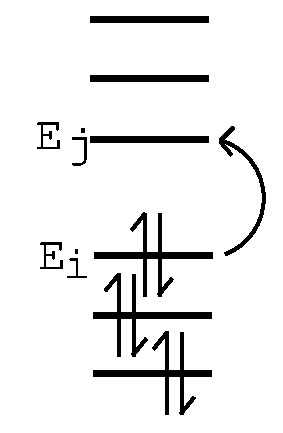
\includegraphics[scale=0.6]{koopman-excite}
\end{center}
\caption{Orbital energies approximating the excitation energy between
two orbitals. The HOMO--LUMO excitation shown would have an excitation energy $E_j-E_i$.} 
\label{koopman-excite}
\end{figure}

Figure \ref{koopman-excite} shows how the orbital energies may be used
approximate excitation energies.

There is one problem with using orbital energies in this fashion. The
orbital energies of the virtual (unoccupied) orbitals actually
corresponds to the states that contain an additional electron. The
orbital energies are computed from interactions where a particle in
the virtual orbitals sees all of the $N_{el}$ electrons, whereas in
reality it should only see $N_{el}-1$ electrons, since it shouldn't
see itself.

\begin{figure}
\begin{center}
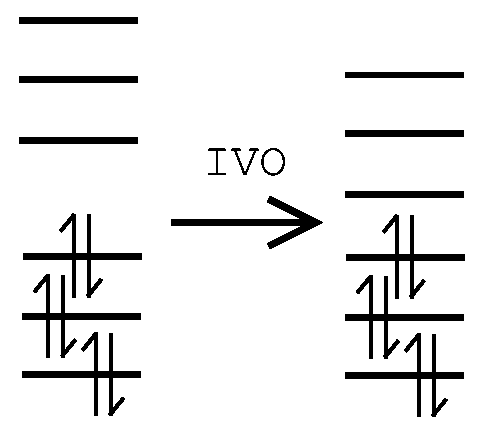
\includegraphics[scale=0.6]{ivo.eps}
\end{center}
\caption{IVO treatment leads to more realistic virtual orbitals and
orbital energies.}  
\label{ivo}
\end{figure}

We can correct this difficulty by using \emph{improved virtual
orbitals} (IVOs). IVOs keep the normal set of occupied orbitals, but
use the state with $N_{el}-1$ electrons for the virtual
orbitals. These orbitals and the associated orbital energies much more
accurately reproduce the proper excited state energies. Figure
\ref{ivo} shows schematically the effect of the ivo treatment.

The following sections detail more rigorous techniques for computing
excited states.

\section{Open Shell Singlet Calculations}
An open-shell singlet (OSS) state is very similar to a triplet state,
except that the two orbitals are singlet paired rather than triplet
paired. A triplet pairing is given by
\begin{equation}
 \Psi_{T} = \phi_{core}\phi_a\phi_b\alpha\alpha
\end{equation}
whereas the open-shell singlet wave function is given by
\begin{equation}
 \Psi_{OSS} = \phi_{core}(\phi_a\phi_b+\phi_b\phi_a)
  (\alpha\beta-\beta\alpha).
\end{equation}
The energy for the triplet wave function is given by $E_{core} +
J_{ab} - K_{ab}$, and the energy of the OSS wave function is given by
$E_{core} + J_{ab} + K_{ab}$.  

OSS wave functions are convenient because they allow standard grand
state programs to be used to compute excited state energies and wave
functions. 

\section{Configuration Interaction Singles}
Open shell singlet descriptions are limited to excited states that can
be described as a single excitation process. Most excited states fall
into this category, but not all do. For those states we may use a
single-excitation configuration interaction approach. Consider a
molecule with occupied orbitals $\phi_a$, $\phi_b$, $\phi_c$,
$\phi_d$, and virtual orbitals $\phi_r$, $\phi_s$, $\phi_t$,
$\phi_u$, and ground state wave function $\Psi$. We write the singly
excited state (also known as a singly excited determinant) when we
take an electron out of occupied orbital $\phi_a$ and put it into
virtual orbital $\phi_r$ as $\Psi_a^r$. We can approximate the excited
state wave function as a linear combination of all of these excited
configurations
\begin{eqnarray}
 \Psi_{CIS} &=& \Psi_a^r + \Psi_a^s + \Psi_b^r + \Psi_b^s + \dots \\
            &=& \sum_i^{occ}\sum_m^{virt} a_{im}\Psi_i^m.
\end{eqnarray}
We wish to find the most optimal linear combination, the one with the
lowest energy. We determine this by forming the Configuration
Interaction (CI) matrix, 
\begin{eqnarray}
 A_{im,jn} = \bracket{\Psi_i^m}{H}{\Psi_j^n}.
\end{eqnarray}
The CI matrix is huge: for a molecule with $n_o$ occupied orbitals and
$n_v$ virtual orbitals, there are $n_o^2n_v^2$ elements, which means
that forming and diagonalizing the matrix can become computationally
expensive very quickly. Typically, only a small range of orbitals
close to the HOMO and LUMO are used as the \emph{active space}, since
realistically, these are the only orbitals that participate in the
excited state to an appreciable degree.

%\section{Time Dependent HF and DFT}

\section{Comparison of results for test systems}
Table \ref{excited} presents results for the methods discussed in this
chapter for a few small molecules whose vertical excitation energies
were well studied experimentally.

\begin{table}
\caption{Vertical excitation energies (in kcal/mol) for a few small
molecules, computed using the techniques discussed in this chapter,
along with experimental results. Computations are performed using the
6-31G** basis set.}
\label{excited}
\begin{center}
\begin{tabular}{cccccc}\hline\hline
Molecule & $\Delta E$ Koopman &  $\Delta E$ IVO &  $\Delta E$ OSS &
  $\Delta E$ CIS &  $\Delta E$ Exp.\\ \hline
Ethylene        & 394.84 & 171.93 & 224.88 & 207.63 & 163.96 \\
Formaldehyde    & 363.90 & 146.65 & 79.25  & 109.92 & 80.71 \\
cis-Butadiene   & 294.21 & 149.87 & 168.15 & 161.67 & 126.60 \\
trans-Butadiene & 285.12 & 144.96 & 173.27 & 165.55 & 136.62 \\
\hline\hline
\end{tabular}
\end{center}
\end{table}

% RPM: repeat table with larger basis?

\section{Nonlinear optical properties of molecules}
Molecules are polarizable: when we put them into an electric field
their electrons reorganize. We can use the dipole moment as a way of
monitoring this polarization
\begin{equation}
 \mu = \mu_0 \alpha E + \frac{\beta E^2}{2!} + \frac{\gamma E^3}{3!} +
  \dots
\label{dipole-nlo}
\end{equation}
The term $\alpha$ is the linear polarizability, $\beta$ is the first
hyperpolarizability, and $\gamma$ is the second
hyperpolarizability. Nonlinear optical effects such as frequency
doubling and second-harmonic generation are a property primarily of
the first hyperpolarizability, so computing this effect efficiently is
of great interest to us.

\begin{figure}
\begin{center}
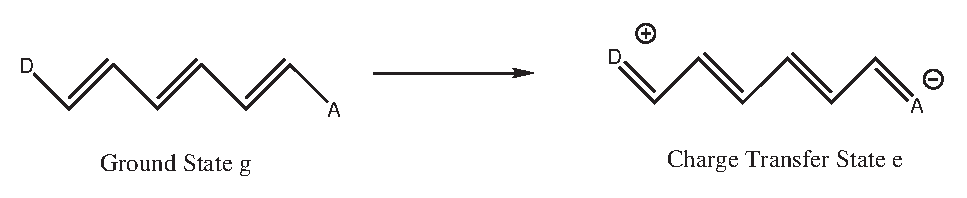
\includegraphics[scale=0.5]{polymer_nlo.eps}
\end{center}
\caption{Two valence bond extremes used to model the polarization
process in a conjugated polymer.}
\label{polymer_nlo}
\end{figure}

Figure \ref{polymer_nlo} shows a two-state model for the polarization
process in a conjugated polymer. Here we consider one neutral valence
bond structure ($g$, for the ground state), and one fully charge
transferred valence bond structure ($e$, for the excited state). Using
the excited state, we can approximate the hyperpolarizability as
\begin{equation}
 \beta \approx \frac{\mu_{ge}^2(\mu_{ee}-\mu_{gg})}{E_{ge}^2}.
\end{equation}
That is, the further apart the two states are, the harder it is to
polarize the molecule. Marder, Perry, and coworkers determined that
the bond-length alternation was a good indication of how far apart in
energy the two states were for conjugated polymers, and based design
of NLO materials on this property.

However, we might wish to determine NLO terms like $\beta$ directly.
The finite field technique computes the dipole moment $\mu(\vec{E})$
at a number of different field strengths and orientations, and use
equation (\ref{dipole-nlo}) to fit the values of $\alpha$, $\beta$,
etc., that reproduce these data. This is a good technique, but
requires many different values of the electric to obtain a good fit.

A better technique, when it is available, is to use \emph{Coupled
Perturbed Hartree Fock} (CPHF) techniques. CPHF computes analytical
derivatives of the energy $\frac{\partial E}{\partial X}$, 
$\frac{\partial^2 E}{\partial X\partial Y}$, etc., with respect to the
electric field strength $\vec(E)$ directly. First derivatives are used
to compute the dipole moment, second derivatives are used to compute
the polarizability, and third and higher derivatives are used to
compute the hyperpolarizabilities. Effectively, in the finite
field technique we are approximating these derivatives. However, the
availablility of this method is dependent upon whether the relevant
analytic derivatives have been programmed for the appropriate
Hamiltonian. 

\section{Suggestions for Further Reading}
Hunt and Goddard \cite{Hunt69} discuss IVO calculations. Szabo and
Ostlund \cite{Szabo82} have a good interaction to CI.  CPHF is
discussed in more detail in \emph{A New Dimension to Quantum
Chemistry} \cite{Yamaguchi94}.





\bibliography{../reference}
\bibliographystyle{unsrt}

\end{document}
